\documentclass[lineno]{JFM-FLM_Au}

\usepackage{amsmath}
\usepackage{upgreek}
\usepackage{bm}
\usepackage{mathtools}

\newcommand{\gd}{{\dot{\bm{\gamma}}}}

\lefttitle{W.C. Reinberger, N.S. Barlow and S.J. Weinstein}
\righttitle{Journal of Fluid Mechanics}

\title{On Self-Similar Viscosity Models for Carreau Boundary Layer Flows}

\author{W. Cade Reinberger\aff{1}, Nathaniel S. Barlow\aff{1} \and Steven J. Weinstein\aff{1}}

\affiliation{\aff{1}[Institution, Department, Address, Country]}

\corresau{W.C. Reinberger, \email{[email address]}}

\begin{document}

\maketitle

\begin{abstract}
   We consider steady boundary layer flows induced by the relative motion of a flat wall and a non-Newtonian fluid under conditions where the wall is moving (Sakiadis flow) and stationary (Blasius flow). These flows admit self-similar ordinary differential equation solutions for Newtonian or power-law viscosity models, but not for generalized-Newtonian viscosity models with a smooth transition between Newtonian and power-law behavior. Since the rates of strain near the wall are high and those away from the wall and far downstream are small, location-dependent power-law and Newtonian behavior is incurred in the same boundary layer flow. Here, we compare flow field predictions from self-similar boundary solutions to those obtained using the Carreau viscosity model and use wall shear-rate predictions as a metric by which viscosity models are compared. To do so, we identify new similarity solutions to the Sakiadis flow and for both shear-thinning and shear-thickening fluids. We find that the wall shear-rates predicted from the power law similarity solution largely agree with those from the Carreau model in regions towards the leading edge of the wall where shear-rates are high; however, there is a finite relative error attributed to differences in the velocity fields away from the wall. No such error is found far downstream along the wall where the flow is Newtonian. We identify a dimensionless criterion that allows both similarity solutions to be combined to approximate Carreau wall shear rate predictions with a quantifiable error.
\end{abstract}

\begin{keywords}
Authors should not enter keywords on the manuscript, as these must be chosen by the author during the online submission process and will then be added during the typesetting process.
\end{keywords}

\section{Introduction}

\hspace{\parindent} A boundary layer describes a thin region adjacent to a wall where viscous effects are important in an otherwise inviscid flow field. The classical boundary layer flow was described by \citet{Blasius}, who in 1908 derived a similarity solution for the steady laminar flow of a Newtonian fluid over a stationary and flat semi-infinite wall. Later, \citet{Sakiadis1961a} extended this framework to model the flow induced by a flat moving wall in an otherwise stationary fluid---a configuration with direct relevance to industrial processes such as liquid film coating \citep{Weinstein2004, TDBlake1994}. The ``Blasius" and ``Sakiadis" boundary layers are mathematically distinct; the nonlinear structure of the governing equations precludes a simple translation of reference frame that relates both problems via a single mathematical solution.

In both flows, the mathematical utility of similarity solutions lies in reducing the governing partial differential equations in two dimensions to an ordinary differential equation (ODE) in a single similarity variable. These classical Newtonian solutions have since been generalized to include fluids with more complex rheological behaviors.  The Ostwald--de Waele power-law model is the most commonly used due to its analytical simplicity, and is expressed as

\begin{equation}
    \mu = K \left|\gd\right|^{\alpha-1}. \label{power_law_constitutive_equation}
\end{equation}


\noindent In (\ref{power_law_constitutive_equation}), $\mu$ is the viscosity, $K$ is the consistency coefficient, $\alpha$ is the power-law exponent, $\gd$ is the rate of strain tensor that depends on velocity gradients, and $|\gd|$ is its magnitude. The Blasius and Sakiadis flows of a power-law fluid were first examined by \citep{Acrivos1960} and \citep{Fox}, respectively. Since then, much literature has focused on the mathematical structure of these flows and their physical applicability \citep{Cortell, Takhar1991, And2007, Pant2004, CoatingFlows}.

The power-law rheological model can, in general, capture shear-thinning or shear-thickening behavior, but fails to reproduce Newtonian behavior at both low and high rates of strain characteristic of fluids encountered in practice (Figure~\ref{fig:rheology}). This is especially relevant to boundary layer flows, where rates of strain near the wall are often high and those away from the wall approach zero.  Furthermore, as the boundary layer grows downstream, the corresponding rates of strain in the boundary layer decrease, so the relative importance of various portions of the rheological profile to the overall flow field may change with location.  Thus, depending on the rheology, the full rheological profile may be accessed in a single boundary layer flow, and the extremities in the profile shown in Figure~\ref{fig:rheology} may be important to the overall flow dynamics.

\begin{figure}
    \centering
    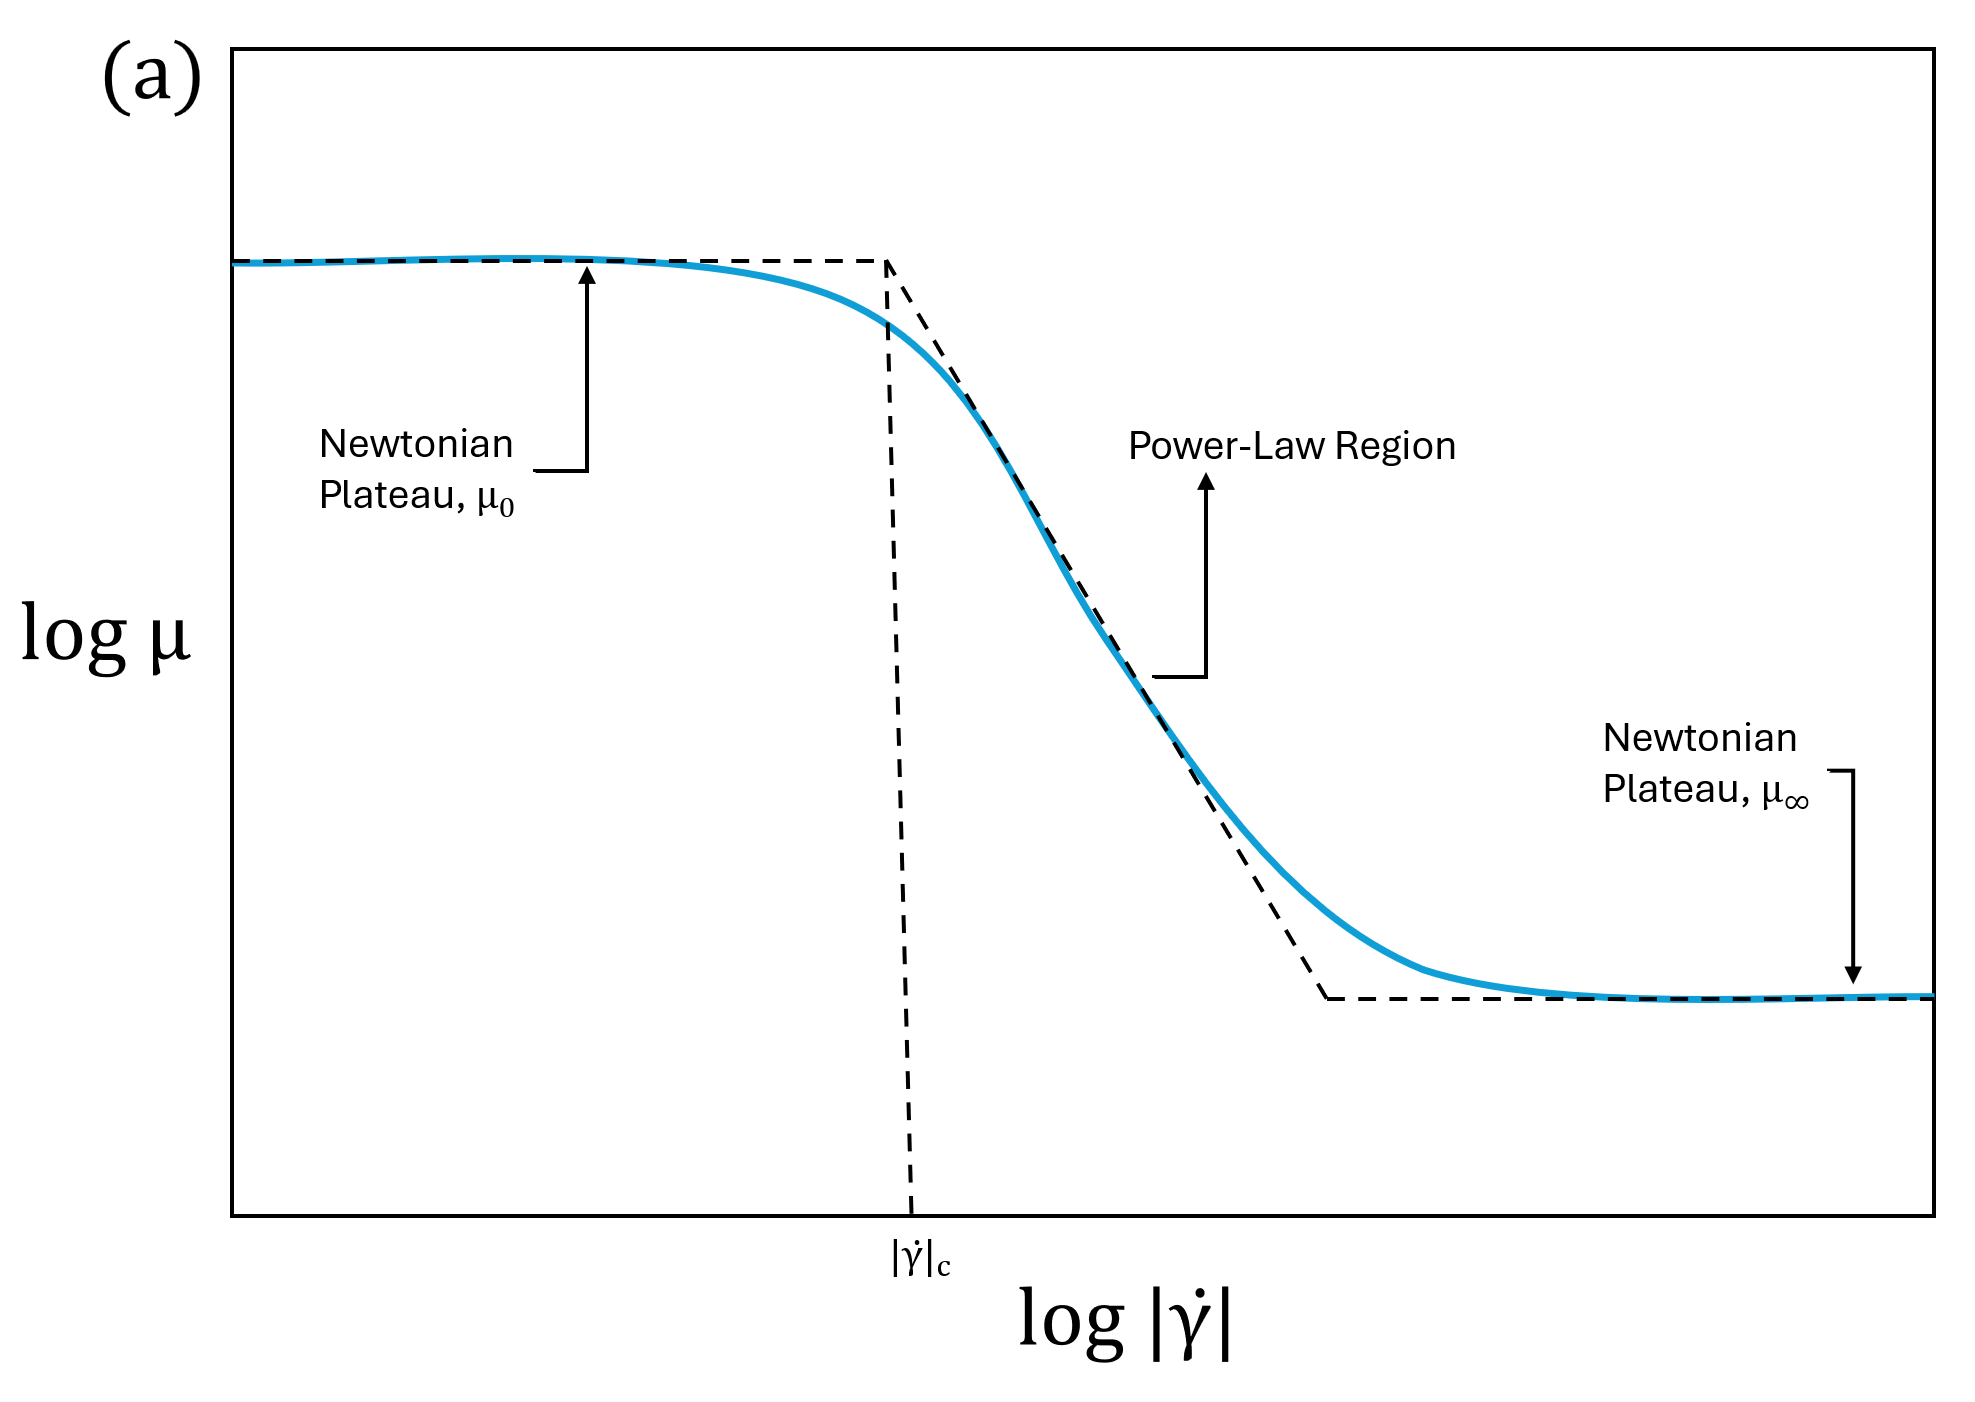
\includegraphics[width=.45\linewidth]{shear_thin_rheo.png}
    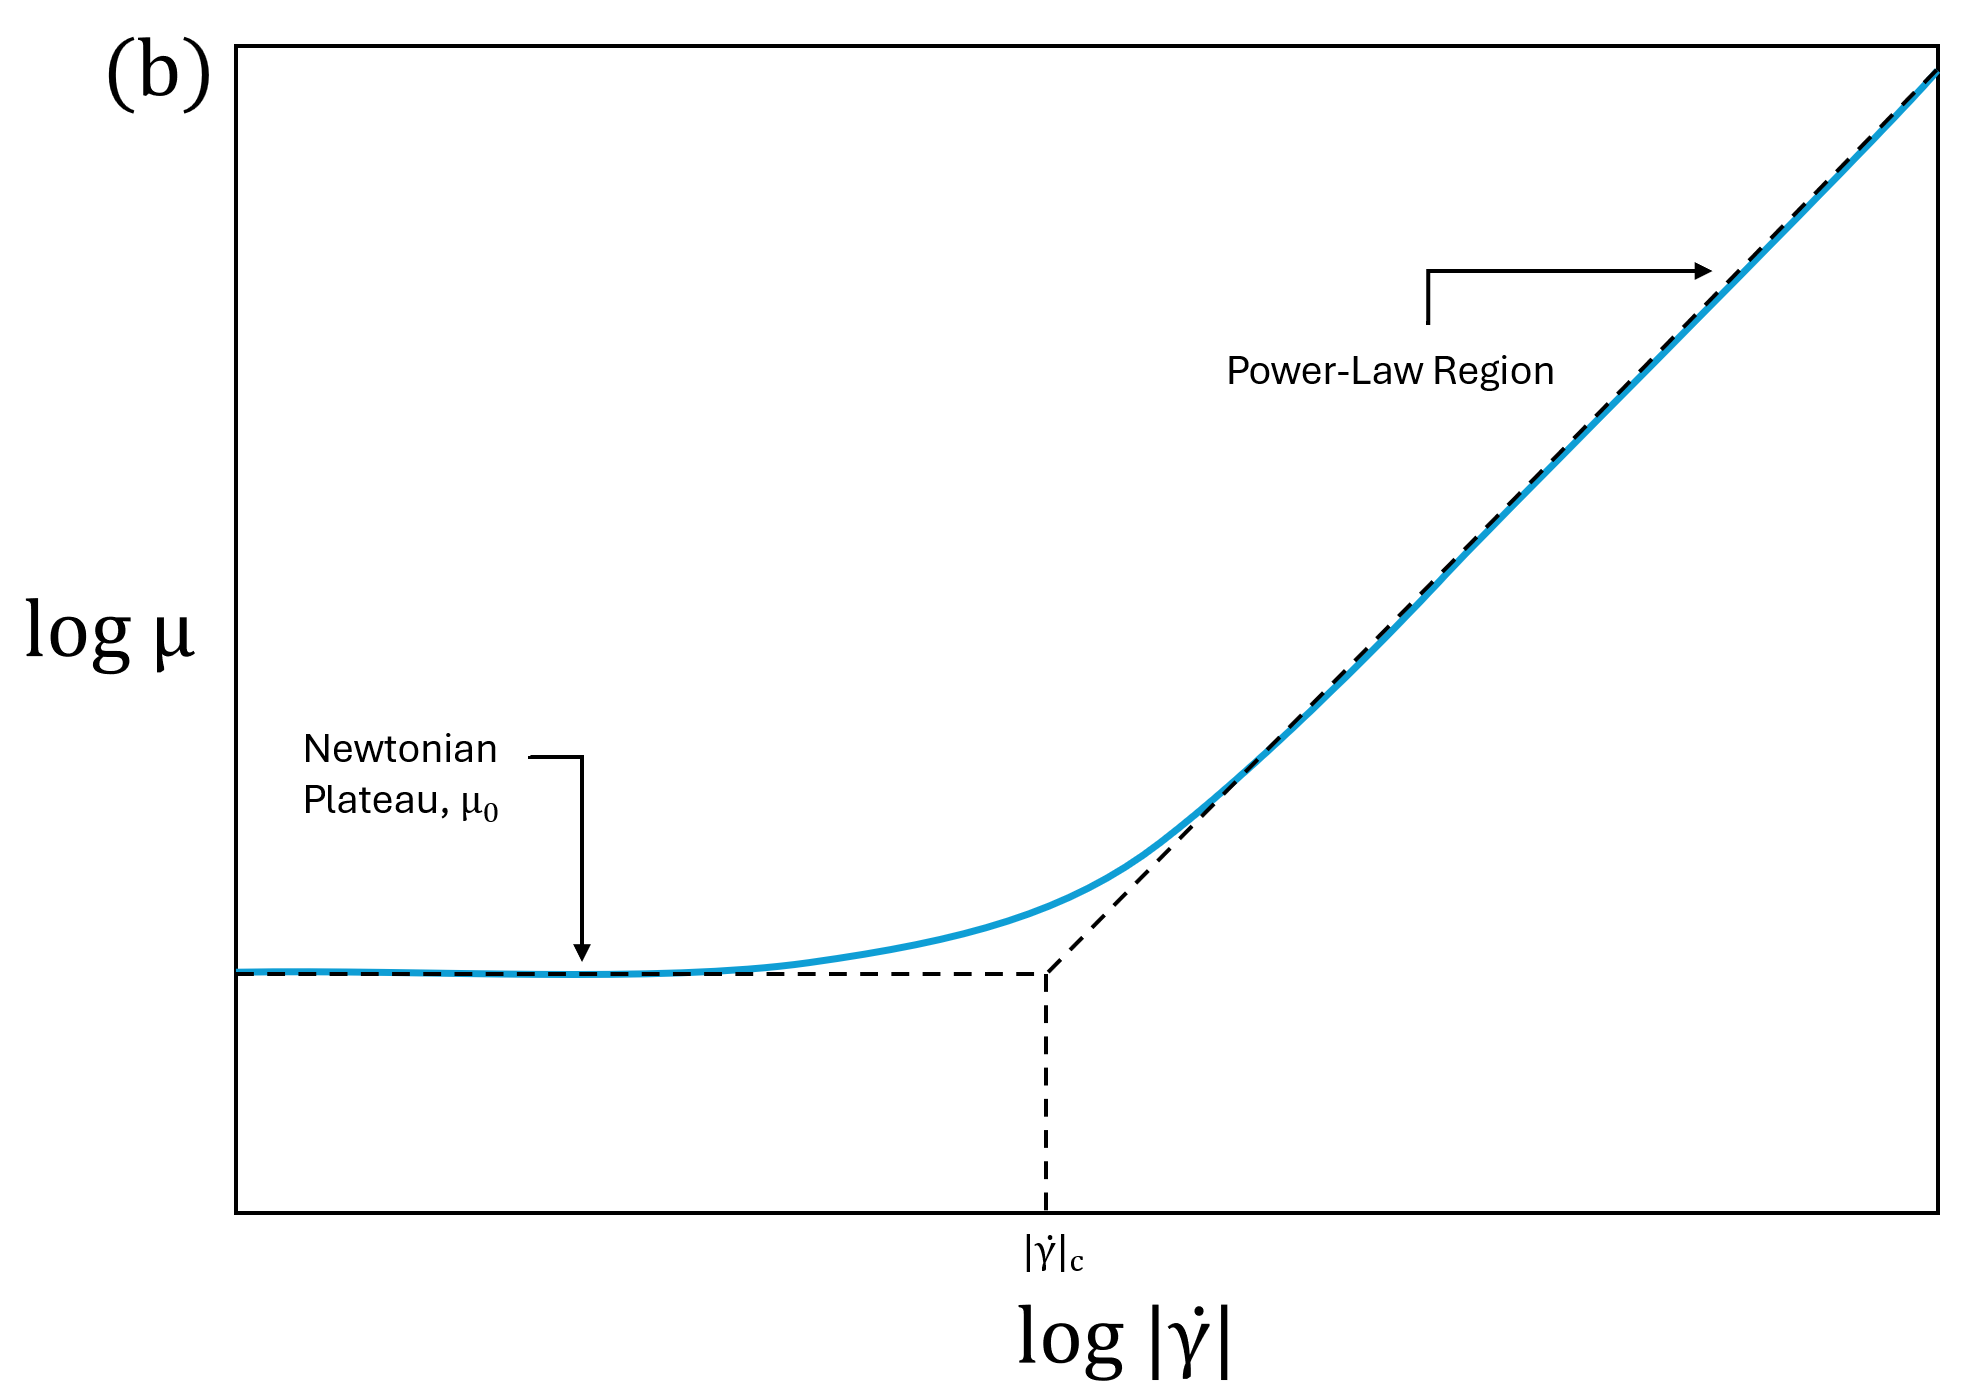
\includegraphics[width=.45\linewidth]{shear_thick_rheo.png}
    \caption{Typical rheological curves showing the dependence of viscosity, $\mu$, on the magnitude of the rate of strain tensor, $|\gd|$.  Solid curves correspond to the Carreau Model from Equation (\ref{carreau_full}). The power-law region has slope $\alpha-1$ on a log-log plot, and the connection between the low-shear and power-law region asymptotes occurs at $|\gd|_c$ in accordance with Equation (\ref{power_law_carreau_limit}). a) Shear-Thinning Behavior. b) Shear-Thickening Behavior.}
    \label{fig:rheology}
\end{figure}

To address these deficiencies, more realistic generalized viscosity relations---such as the Carreau model---have been used in previous studies of Sakiadis and Blasius boundary layer flows \citep{PANTOKRATORAS, Griffiths}.  The Carreau model incorporates both shear-dependent power-law behavior and its asymptotic Newtonian limits, providing a smooth transition between low-shear and high-shear regimes as shown in Figure~\ref{fig:rheology}; it can thus fully characterize many typical experimentally measured viscosity curves. The Carreau model is expressed as

\begin{equation}
    \mu = \mu_\infty + (\mu_0 - \mu_\infty)\left(1 + (\lambda|\gd|)^2\right)^{(\alpha-1)/2} \label{carreau_full}
\end{equation} where $\mu_0$ is the Newtonian viscosity at low strain-rate magnitudes ($|\gd| \ll 1/\lambda$), $\mu_\infty$ is the Newtonian viscosity at high strain-rate magnitudes ($|\gd| \gg 1/\lambda$), and $\lambda$ is a relaxation time parameter.  In many practical flow fields, the high strain-rate Newtonian plateau is not reached, and rheological data may be well fit by setting $\mu_\infty = 0$. In this paper, we restrict attention to this situation. Under these circumstances, the Carreau model becomes \begin{subequations}
\begin{equation}
    \mu = \mu_0\left(1 + (\lambda|\gd|)^2\right)^{(\alpha-1)/2}. \label{carreau_simplified}
\end{equation} From this, it is straightforward to deduce the low-shear and power-law asymptotes shown in Figure~\ref{fig:rheology} as
 \begin{equation} \mu \sim \mu_0 ~~~~(|\gd| \to 0) \hphantom{\sum\sum} \mu \sim \mu_0\lambda^{\alpha-1} |\gd|^{\alpha-1} ~~~~(|\gd| \to \infty). \label{carreau_asymptotes} \end{equation}
The intersection between these asymptotes defines the critical rate of strain, $|\gd|_c$, for the onset of shear thinning as \begin{equation} |\gd|_c = \frac{1}{\lambda}. \label{power_law_carreau_limit}\end{equation} Thus, the parameter $\lambda$ characterizes the onset of shear thinning through (\ref{carreau_asymptotes}) (see Figure~\ref{fig:rheology}), and the consistency coefficient $K$ in the limiting power-law model may be expressed in terms of Carreau parameters by comparing (\ref{power_law_carreau_limit}) and (\ref{power_law_constitutive_equation}) as \begin{equation}
    K = \mu_0 \lambda^{\alpha-1}. \label{carreau_power_law_limit_constistency_parameter}
\end{equation} \end{subequations} The connection between the Carreau and power-law models is thus made clear via (\ref{carreau_power_law_limit_constistency_parameter}). Note that the power-law model (\eqref{power_law_constitutive_equation} with \eqref{carreau_power_law_limit_constistency_parameter}) and the Carreau model (\eqref{carreau_full} or \eqref{carreau_simplified}) both reduce to a constant Newtonian viscosity for $\alpha=1$, i.e. \begin{equation}
    \mu = \mu_0 ~~~~\forall ~ |\gd|. \label{newtonian_viscosity}
\end{equation}

The power-law model is often utilized in fundamental research studies to examine phenomenologically how shear-dependent viscosity affects a flow field.  To date, the authors are unaware of any systematic study demonstrating the efficacy of the power-law model in predicting boundary layer flow structure compared with more realistic viscosity models. One feature of more realistic models---such as the Carreau model examined here---is that they do not admit similarity solutions for the Blasius and Sakiadis flows, which complicates both analysis and computation.  One aim of the present work is to assess the extent to which the predictions of simpler, self-similar models provide adequate descriptions of Blasius and Sakiadis flows compared with those using the Carreau model.  To do so, we focus on wall shear as a metric of comparison, but also examine differences in velocity profiles that arise between these models.

The power-law model provides an incomplete description of fluid rheology (again, refer to Figure~\ref{fig:rheology}), and there are some notable changes in the mathematical structure of boundary layer flows that arise upon changing the value of the power-law exponent $\alpha$ in \eqref{power_law_constitutive_equation}.  This change of structure is relevant to our comparative study of power-law and Carreau model results, and we recount some of that literature here.  For Blasius boundary layers, it is well-known that an infinitely differentiable velocity profile is obtained for shear-thinning fluids ($\alpha < 1$), but the velocity profile loses smoothness for shear-thickening fluids ($\alpha>1$): the velocity profile has a discontinuity in its fifth derivative, although it is continuous through its fourth \citep{Zhizhin1978-us, Pavlov1982-qh}. \citet{Dabrowski} suggest that this discontinuous solution structure in the power-law model arises from a breakdown in the boundary layer equations far from the wall when the viscosity is suitably small.  They demonstrate that a continuous solution can be obtained by introducing a ``viscous diffusion layer" that incorporates viscous derivatives neglected in the boundary layer equation. In this paper, we demonstrate that the Carreau model---a viscosity model with built-in Newtonian limits---yields a continuous solution for all $\alpha$ without the need to invoke modifications to the boundary layer approximation itself.

Previous work on the Sakiadis boundary layer using a power-law model indicates that no solution exists for all shear-thickening fluids ($\alpha > 1$) and for some shear-thinning fluids ($\alpha < 1/2$) \citep{Fox, NonNewtonian}. These results are based on the fact that the dimensionless stream function, $f$, satisfies $\text{d}f/\text{d}\eta \to 0$ as $\eta \to \infty$, where $\eta$ is the similarity variable (corresponding to large distances from the wall). Previous work assumes an asymptotic form where $f \sim C + h(\eta)$ with $C$ a constant and $h(\eta) \ll C$ as $\eta \to \infty$. The statement that there are no solutions for $\alpha < 1/2$ is based on the fact that this assumption is not self-consistent for $\alpha < 1/2$.  However, in this paper we demonstrate that solutions do exist in the form $f \sim H(\eta + J)^p$ as $\eta \to \infty$, where $H$ and $J$ are constants and $0<p<1$.  Furthermore, solutions \textit{do} exist for shear-thickening flows ($\alpha > 1$) with $f$ identically constant for $\eta$ sufficiently large, and these solutions are \textit{not} continuously differentiable in their fifth derivative; this structure is analogous to that found in the Blasius problem for a shear-thickening power-law fluid \citep{Zhizhin1978-us, Pavlov1982-qh}. We show that these additional power-law boundary layer solutions yield wall-shear stress predictions that agree with those from the Carreau model at locations along the wall where significant shear-dependent behavior is evident.

The organization of the paper is as follows. In Section 2, the formulations of the Sakiadis and Blasius problems are provided for Newtonian, power-law, and Carreau model fluids. Although the Carreau constitutive law does not admit a similarity solution, we make use of previous literature \citep{Griffiths} to recover a one-parameter family of ODE solutions that describe the flow at each streamwise location along the wall. In Section 3, we examine the new power-law solutions for the Sakiadis flow for $\alpha < 1/2$ and $\alpha > 1$. Section 4 provides a comparison between the wall shear-rates predicted for a Carreau fluid with those predicted from Newtonian or power-law similarity solutions, over a wide range of flow conditions. Section 5 discusses the efficacy of self-similar predictions to approximate Carreau values for wall-shear, as well as comparisons of velocity profiles. Closing comments and conclusions are provided in section 6.

\section{Formulation}

\subsection{Boundary Layer Equations}

 \hspace{\parindent} We consider the steady boundary layer flow induced by the motion between a fluid and an infinite flat wall as shown in Figure~\ref{flow_setups}. There are two configurations that we examine: the \textit{Blasius} boundary layer induced by a moving fluid over a stationary wall (Figure~\ref{flow_setups}a), and the \textit{Sakiadis} boundary layer induced by a moving wall in an otherwise stationary fluid (Figure~\ref{flow_setups}b). As indicated, the $x$ coordinate is oriented along the wall, the $y$-direction is perpendicular to the wall; the flow is invariant in the $z$-direction (not shown---oriented out of Figure~\ref{flow_setups}). Corresponding velocities in the $x$ and $y$ directions are $u_x$ and $u_y$, respectively.  In the Blasius configuration, $u_x=U$ is the velocity of the fluid away from the wall ($y \to \infty$); while in the Sakiadis problem, $u_x=U$ is the velocity of the wall ($y=0$).  In both problems, the pressure field is constant and plays no role in the flow dynamics.

 \begin{figure}
    \centering
    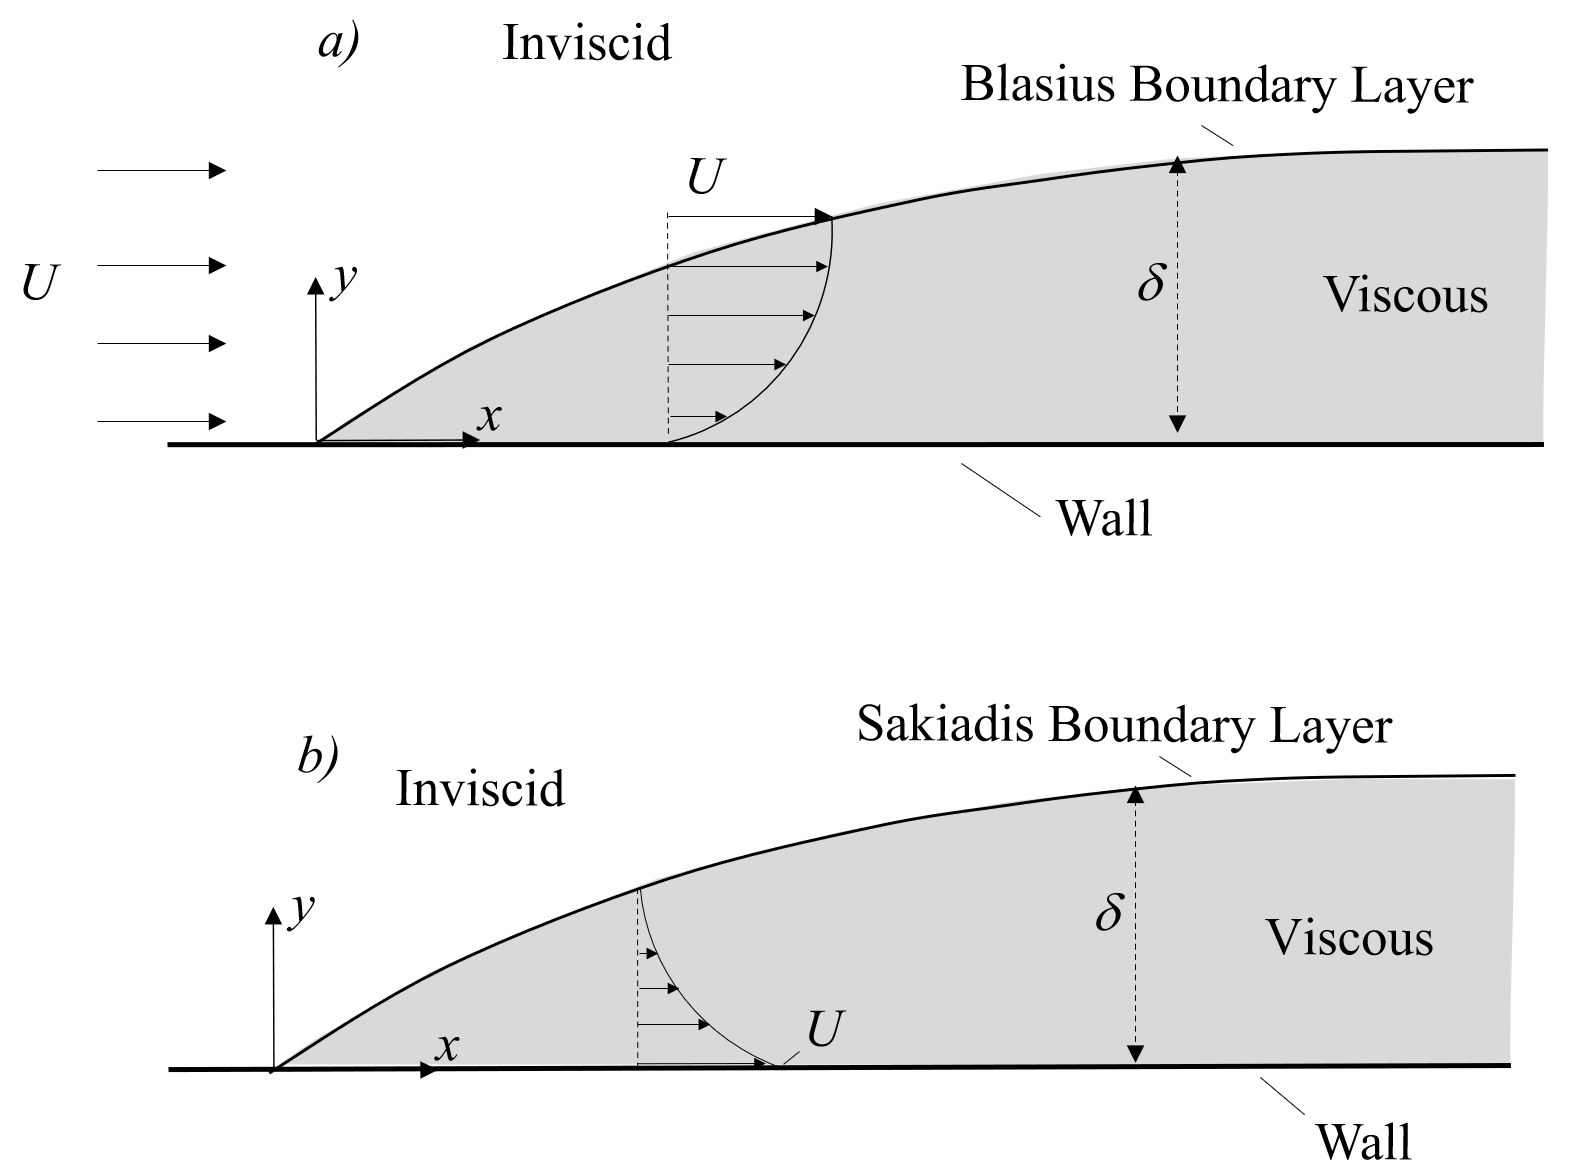
\includegraphics[width=.95\linewidth]{schem_fixed.png}
    \caption{Schematics depicting boundary layer flows along a flat wall.  a) Blasius, b) Sakiadis.  Here, $U$ is the velocity of the oncoming fluid or wall and $\delta$ is the boundary layer thickness that increases with distance downstream, $x$.}
    \label{flow_setups}
\end{figure}


In accordance with the boundary layer approximation, the flow in Figure~\ref{flow_setups} is essentially inviscid away from the wall, and the effects of viscosity are confined to a thin region---a boundary layer---near the wall.  As such, velocity variations in the $y$ direction are large compared with those in the $x$ direction, and viscous stresses across the boundary layer dominate.  As a result, the boundary layer approximation to the equations of motion is \citep{Schlichting}

\begin{subequations} \label{blsystem}
    \begin{align}
        &\frac{\partial u_x}{\partial x} + \frac{\partial u_y}{\partial y} = 0 \label{conteqinbl}\\
        & \rho \left\{ u_x \frac{\partial u_x}{\partial x} + u_y \frac{\partial u_x}{\partial y} \right\} = \frac{\partial \tau_{yx}}{\partial y} \label{blmomeq}
    \end{align} where $\rho$ is the density of the fluid and the relevant component of the stress tensor is given as \begin{align}
        \tau_{yx} = \mu \frac{\partial u_x}{\partial y},~~~~\mu = \mu(|\gd|),~~~~|\gd| = \left|\frac{\partial u_x}{\partial y} \right|. \label{stress_tensor_component}
    \end{align} In (\ref{stress_tensor_component}), a generalized Newtonian form for the viscosity $\mu$ has been assumed, as it is a function of the magnitude of the rate of strain as indicated. Consistent with the configurations shown in Figure~\ref{flow_setups}, the boundary conditions are
\begin{align}
\mathmakebox[7em][l]{\text{Location}}
\mathmakebox[12em][l]{\text{Blasius}}
\mathmakebox[12em][l]{\text{Sakiadis}}
\nonumber\\
\mathmakebox[7em][l]{y=0}
\mathmakebox[12em][l]{u_x=0,\quad u_y=0}
\mathmakebox[12em][l]{u_x=U,\quad u_y=0}\\
\mathmakebox[7em][l]{y\to\infty}
\mathmakebox[12em][l]{u_x\to U}
\mathmakebox[12em][l]{u_x\to 0}
\end{align}
\end{subequations}

In this paper, we consider specific forms of $\mu(|\gd|)$ in (\ref{stress_tensor_component}) for power-law \eqref{power_law_constitutive_equation}, Carreau \eqref{carreau_simplified}, and Newtonian \eqref{newtonian_viscosity} models.  Regardless of viscosity model, the system (\ref{blsystem}) is expressed in terms of a streamfunction $\psi$, satisfying $u_x = \partial \psi/\partial y$ and $u_y = -\partial \psi/\partial x$. As discussed in the following sections 2.2 and 2.3, these equations are then further simplified via similarity transform methods.

\subsection{Power-Law and Newtonian Fluids}

\hspace{\parindent} For a power-law fluid, the PDE system (\ref{blsystem}) admits a similarity solution using the substitutions \begin{subequations}
    \begin{equation}
        \eta = y\left(\dfrac{\rho U^{2-\alpha}}{Kx}\right)^{1/(\alpha+1)}
    \end{equation}
    \begin{equation}
        f_p(\eta; \alpha) = \frac{\eta \psi}{Uy}
    \end{equation}
\end{subequations} that yields an ODE for $f_p$ given by \begin{subequations} \begin{equation}
     \alpha(\alpha+1)f_p''' + f_pf_p''|f_p''|^{1-\alpha} = 0, \label{power_law_ode_only} \end{equation} with boundary-conditions given as \begin{equation} f_p(0; \alpha)=0~~~~f_p'(0; \alpha)=0~~~~f_p'(\infty; \alpha) \to 1 ~~~~ (\mathrm{Blasius}) \end{equation} and \begin{equation} f_p(0; \alpha)=0~~~~f_p'(0; \alpha)=1~~~~f_p'(\infty; \alpha) \to 0 ~~~~ (\mathrm{Sakiadis}). \label{power_law_sak_bcs}\end{equation}  \label{power_law_ode_general} \end{subequations} The associated streamwise velocity component, $u_x$, may be extracted as \begin{equation} u_x = U f_p'(\eta; \alpha). \label{streamwise_velocity_expression} \end{equation}The dimensional expression for the wall shear rate for a power-law fluid, $\tau_p$, is likewise extracted from the solution for $f_p$, and is expressed as \begin{subequations} \begin{equation}
    \tau_p = K \left(U \left|f_p''(0; \alpha)\right|\left(\dfrac{\rho U^{2-\alpha}}{Kx} \right)^{1/(\alpha+1)}  \right)^\alpha .\label{pl_dimensional_wall_shear}
\end{equation} In (\ref{pl_dimensional_wall_shear}), note that $f_p''(0; \alpha)<0$ for the Sakiadis flow, and $f_p''(0; \alpha)>0$ for the Blasius flow. The analogous expressions for a Newtonian fluid can be obtained from (\ref{pl_dimensional_wall_shear}) by inserting $\alpha=1$ and $K=\mu_0$ in accordance with \eqref{power_law_constitutive_equation} to yield \begin{equation}
    \tau_n = |f_p''(0; 1)| \sqrt{\dfrac{\rho \mu_0 U^3}{x}} \label{newtonian_dimensional_wall_shear}
\end{equation} \end{subequations} where the subscript $n$ denotes the Newtonian wall shear rate.

\subsection{Carreau Fluid}

\hspace{\parindent} Unlike Power Law or Newtonian fluids, the boundary layer equations for a Carreau fluid do not admit a self-similar solution. In general, this necessitates a numerical solution of the governing PDE system \eqref{blsystem} (using $\mu$ in \eqref{carreau_simplified}) for Blasius or Sakiadis configurations. However, following the approach of \citet{Griffiths}, one can transform the governing system into an 1-parameter family of ODEs via the similarity variable used for a Newtonian fluid.  In this form, the $x$-dependence does not disappear completely, but arises solely as a parameter in the problem.  This necessitates that the ODE be solved at each streamwise location $x$ in Figure 2.

As such, we define a dimensionless streamfunction for the Carreau model, $f_c$, as\begin{equation} f_c = \psi \sqrt{\dfrac{\rho}{\mu_0 x U}} \label{sim_pt1}\end{equation} and we likewise define the similarity coordinate \begin{equation} \eta = y \sqrt{\dfrac{\rho U}{\mu_0 x}}. \label{sim_pt2} \end{equation} Substituting (\ref{sim_pt1}) and (\ref{sim_pt2}) into (\ref{blsystem}), one obtains an ODE with an $x$-dependent parameter. Defining the local parameter $\delta$ as \begin{equation}
    \delta = \frac{\lambda^2 U^3 \rho}{\mu_0 x}, \label{delta_definition}
\end{equation}  one obtains \begin{subequations}
    \begin{align}
       & \left(1+\alpha\delta f_c''^2 \right) \left(1+\delta f_c''^2 \right)^{(\alpha-3)/2} f_c''' + \frac{1}{2}f_cf_c'' = 0 \label{carreau_ode_form_ode} \\ &f_c(0; \alpha)=0~~~~f_c'(0; \alpha)=0~~~~f_c'(\infty; \alpha) \to 1 ~~~~ (\mathrm{Blasius})\label{carreau_ode_form_blasius_bcs}  \\
    & f_c(0; \alpha)=0~~~~f_c'(0; \alpha)=1~~~~f_c'(\infty; \alpha) \to 0 ~~~~ (\mathrm{Sakiadis}). \label{carreau_ode_form_sakiadis_bcs}
    \end{align} \label{carreau_ode_form_full_system} \end{subequations}
\noindent For a given set of rheological parameters, the ODE system (\ref{carreau_ode_form_full_system}) has a single free parameter, $\delta$, that changes with distance $x$ downstream (Figure~\ref{flow_setups}). Thus, by solving the system (\ref{carreau_ode_form_full_system}) for an appropriate array of $\delta$ values spanning the desired $x$-domain, the whole flow field may be determined without considerable computational effort. As indicated in \eqref{delta_definition}, the $x$-dependent parameter $\delta$ incorporates the constant $\lambda$ present in the Carreau viscosity model \eqref{carreau_full}.  It is apparent from the location of $\delta$ in (\ref{carreau_ode_form_ode}) that it acts as an effective relaxation time---its inverse relationship with $x$ indicates that the magnitude of shear-dependent behavior decreases downstream.  This observation is physically intuitive, as it is consistent with the physics of a growing boundary layer in the original $x$-$y$ domain (Figure~\ref{flow_setups}), and indicates that velocity gradients decrease accordingly. Using the solution to \eqref{carreau_ode_form_full_system}, the dimensional expression for the wall shear, $\tau_{c}$, is expressed as \begin{equation}
    \tau_{c} = \sqrt{\dfrac{\rho  \mu_0U^3}{ x}}f_c''\left(0; \delta\right)\left(1 + \delta f_c''\left(0; \delta\right)^2  \right)^{(\alpha-1)/2} .\label{carreau_wall_shear_dimensional_expression}
\end{equation}

\subsection{Numerical Solution}

\hspace{\parindent} To solve the relevant boundary value problems for power-law, Newtonian (power-law with $\alpha=1$), or Carreau rheologies from Sections 2.2 and 2.3, we convert the relevant boundary value problems (\ref{power_law_ode_general}) and (\ref{carreau_ode_form_full_system}) into initial value problems by imposing a value of $f_c''(0; \delta)$.  We then truncate the domain to a length $L$, and use a standard RK45 integrator with shooting to meet the $y\to\infty$ boundary conditions in \eqref{carreau_ode_form_sakiadis_bcs}---now imposed at $y=L$. The length $L$ is then increased and the calculation repeated until convergence is achieved to within an absolute error tolerance of $10^{-6}$.

\section{New Sakiadis Solutions for Power-Law Fluids}

\hspace{\parindent} To facilitate comparison with the Carreau model solution for Blasius and Sakiadis flows, the self-similar solution to the ODE (\ref{power_law_ode_general}) for a power-law fluid is necessary. Power-law solutions for Blasius flows are well-known for all values of $\alpha>0$. For the case of a Sakiadis flow, however, \citet{Fox} and \citet{NonNewtonian} indicated that no solutions exist for two distinct classes of power-law fluids: those with $\alpha < 1/2$ and $\alpha > 1$. This conclusion is based on an analysis of one particular asymptotic form of the Sakiadis flow away from the wall. In what follows, we show that alternative asymptotic forms are possible that enable power-law solutions to be obtained in these previously excluded regimes of $\alpha$.

\subsection{Shear-Thinning Fluids ($\alpha < 1/2$)}


\hspace{\parindent} For the power law model in the Blasius configuration, a solution exists for all $\alpha < 1$ with the property that $f \sim \eta$ as $\eta \to \infty$. In the Sakiadis case, however, the existence of a power-law solution is only known for $\alpha \in (1/2, 1]$.  Given the similarities between the ODEs governing Blasius and Sakiadis flows, this inability to obtain a power-law solution outside of this range is not anticipated.  We resolve this non-analogous behavior in what follows.

For a Sakiadis flow, the dimensionless streamfunction $f_p(\eta; \alpha)$ satisfies (\ref{power_law_ode_only}) with boundary conditions (\ref{power_law_sak_bcs}). The Newtonian Sakiadis equation ($\alpha=1$) admits a solution having asymptotic behavior that can be derived assuming $f_p(\eta; 1) \to C$, whence the method of dominant balance yields\begin{equation} f_p(\eta; 1) \sim C + Ge^{-C\eta/2} \hphantom{\sum} \text{as}~~ \eta \to \infty,\end{equation} with $C$ and $G$ constants \citep{GenMeth}. For shear-thinning fluids with $1/2 < \alpha < 1$, an analogous dominant balance subject to the same assumption leads to \begin{equation}
    f_p\left(\eta; \alpha\right) \sim C + D\left(1 + E\eta \right)^{^{\frac{2\alpha-1}{\alpha-1}}} \hphantom{\sum} \mathrm{for}~~ \frac{1}{2}<\alpha<1, ~~ \mathrm{as}~~\eta \to \infty, \label{sakiadis_shear_thinning_classical_asymptotic}
\end{equation} with $C, D$, and $E$ constants that may depend on $\alpha$; as is standard for dominant balance problems, these constants remain arbitrary when only the asymptotic behavior is assessed. Note that this form breaks the dominant-balance assumption when the leading constant term $C$ becomes asymptotically subdominant to the second term as $\eta \to \infty$, which happens for $\alpha$ outside the range indicated in (\ref{sakiadis_shear_thinning_classical_asymptotic}). The conclusion that there is no solution for $\alpha<1/2$ in \citet{Fox} and \citet{NonNewtonian} is based on the asymptotic form (\ref{sakiadis_shear_thinning_classical_asymptotic}); in what follows, we show that another dominant balance can be satisfied that leads to an expanded range of admissible $\alpha$ values.

Indeed, the boundary condition (\ref{power_law_sak_bcs}) does not require \textit{a priori} that $f_p \sim C$ as $\eta \to \infty$. Rather, a solution to equation (\ref{power_law_ode_only}) that satisfies equation (\ref{power_law_sak_bcs}) exists and admits the asymptotic form \begin{subequations} \begin{equation}
    f_p\left(\eta; \alpha \right) \sim H \left(\eta+J\right)^{p} \hphantom{\sum\sum} \mathrm{for}~~0 < \alpha < \dfrac{1}{2}~~ \mathrm{as}~~ (\eta \to \infty),
\end{equation} where \begin{equation} p = \dfrac{1-2\alpha}{2-\alpha} \end{equation}  and \begin{equation}
    H = \left(\dfrac{\alpha(\alpha+1)(2-p)}{p^{1-\alpha}(1-p)^{1-\alpha}}\right)^{^{\frac{1}{2-\alpha}}}.
\end{equation} \label{power_law_sakiadis_new_asymptotic} \end{subequations} \noindent In (\ref{power_law_sakiadis_new_asymptotic}), $J$ is an arbitrary constant that reflects the autonomous nature of the ODE (\ref{power_law_ode_general}).

To examine the properties of this solution, we consider the boundary value problem (BVP) system (\ref{power_law_ode_general}) as arising from a corresponding initial value problem (IVP). For a given value of $\alpha$, one may write $f_p''(0; \alpha)=\kappa$ and vary the initial condition $\kappa$ to examine $f'$ as $\eta \to \infty$. In so doing, we find that for $\kappa$ greater than a critical value $\kappa=\kappa_p$, solutions for $f_p$ are monotonically increasing for all $\eta \geq 0$, while they are nonmonotone and eventually decrease with $\eta$ for $\kappa<\kappa_p$. Figure~\ref{fig:shooting} shows this structure, indicating that the solution corresponding to $\kappa=\kappa_p$ is a separatrix delineating the two asymptotic behaviors (see dashed line in Figure~\ref{fig:shooting}). At $\kappa=\kappa_p$, the solution smoothly approaches $f_p' \to 0$ as $\eta \to \infty$. This value of $\kappa_p$ is the unique initial value with this property for $f_p'$ as $\eta \to \infty$, and we therefore propose that it represents the correct solution for $\alpha<1/2$.

\begin{figure}
    \centering
    
\includegraphics[width=0.6\linewidth]{fig3.eps}
    \caption{Shooting solutions of the Sakiadis problem obtained by considering (\ref{power_law_ode_only}) as an IVP with various values of $f_p''(0; \alpha)=\kappa$ for $\alpha = 0.3$. The solution to the boundary value problem (\ref{power_law_ode_general}) for $\kappa=\kappa_p$ is indicated with a dashed curve, and corresponds to a separatrix between shooting solutions with distinctive behaviors. Solutions above the separatrix orbit are shown in blue, and solutions below it are shown in green; the latter obtain a local maximum in $[0, L]$. For $\kappa$ above the true value of $\kappa_p$ the solutions (shown in blue) obtain no local maximum anywhere on $[0, \infty)$.}
    \label{fig:shooting}
\end{figure}

The separatrix solution is found numerically to match the asymptotic behavior (\ref{power_law_sakiadis_new_asymptotic}) as shown in Figure~\ref{fig:new_asymptotic}. Furthermore, we note that the behavior of the dimensionless wall-shear $f_p''(0; \alpha)$ varies continuously with $\alpha$ as $\alpha \to 1/2^-$ as shown in Figure~\ref{fig:kappavsalpha}; that is, solutions corresponding to the switch in asymptotic forms from (\ref{sakiadis_shear_thinning_classical_asymptotic}) and (\ref{power_law_sakiadis_new_asymptotic}) yield continuous results. Finally, numerical results confirm that the solution to the power-law Sakiadis equation yields a computed value of $\kappa_p$ that closely follows the high-shear limit for wall shear observed in the Carreau model, to be described in Section 4. Taken together, the consistency of the wall-shear rate and asymptotic behavior predictions with Carreau predictions justifies the conclusion that new admissible Sakiadis power-law solutions have been found for $\alpha<1/2$.

\begin{figure}
    \centering
    
\includegraphics[width=0.6\linewidth]{new_thinning_asymptotic.eps}
    \caption{Log-log plot of the separatrix solution $f_p(\eta; \alpha)$ in Figure \ref{fig:shooting} for the Sakiadis boundary layer for a power-law fluid with $\alpha = 0.1$. The dashed line shows the predicted asymptotic form $f_p \sim H(\eta +J)^p$ from (\ref{power_law_sakiadis_new_asymptotic}) (for simplicity, $J$ is set to 0 for the plot, since it does not change the asymptotic to first order), and the solid line is the numerical solution to (\ref{power_law_ode_general}).}
    \label{fig:new_asymptotic}
\end{figure}

\begin{figure}
    \centering
    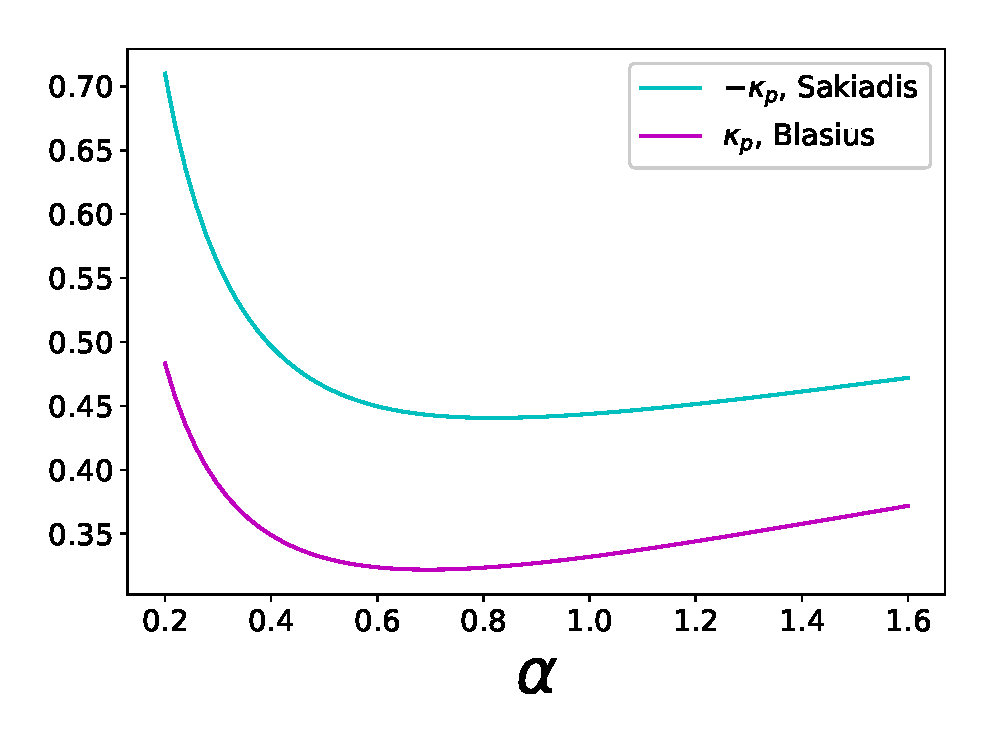
\includegraphics[width=\textwidth]{fig5.eps}
    \caption{Dimensionless wall-shear coefficient $\kappa_p=f_p''(0; \alpha)$ for power-law fluids as a function of $\alpha$ for a) the Blasius boundary layer b) the Sakiadis boundary layer. Note the values vary continuously between previously known solutions for $1/2<\alpha\leq1$ and new solutions to the Sakiadis problem for $\alpha < 1/2$ and $\alpha > 1$.}
    \label{fig:kappavsalpha}
\end{figure}


\subsection{Shear-Thickening Fluids ($\alpha > 1$)}

\hspace{\parindent} When $f_p \to C$ is also assumed for shear-thickening ($\alpha>1$) power-law fluids, the asymptotic equation (\ref{sakiadis_shear_thinning_classical_asymptotic}) again indicates that no solution satisfies the dominant balance, since the second term is not subdominant to the first \citep{Bender}. However, in this case, we once again find that there exists another class of power-law solutions to the Sakiadis problem (\ref{power_law_ode_general}). Insight can be gained here by analogy to the Blasius problem and its well-known structure. For a power-law fluid in the Blasius boundary layer, it is known that the dimensionless streamfunction admits a ``singular solution'' that is $C^4$ but not $C^5$ (four but not five times continuously differentiable) at a distinguished ``singular'' point along the solution curve \citep{Zhizhin1978-us, Pavlov1982-qh}.\footnote{We note the $|f_p''|^{2-\alpha}$ term in the ODE (\ref{power_law_ode_only}) is Lipschitz when $\alpha \leq 1$ but not when $\alpha >1$, in the shear-thickening case. Thus, the usual existence and uniqueness theorem (Picard--Lindel\"{o}f) does not apply when the solution to (\ref{power_law_ode_only}) is viewed as an initial value problem, which allows the singular structure described to occur. This is necessary because at the singular point the solution to the associated IVP is non-unique, as continuing the constant solution for $\eta \to C_1^-$ would yield a solution to the ODE (\ref{power_law_ode_only}), but not the associated boundary conditions (\ref{power_law_sak_bcs}).}

Similarly to the shear-thinning case ($\alpha < 1$), numerical results for $\alpha > 1$ indicate a separatrix solution exists between monotone and nonmonotone solutions as shown in Figure~\ref{fig:shooting_thick}; this separatrix structure is analogous to that for $\alpha<1/2$ in Figure~\ref{fig:shooting} (see dashed line). Here, however, the streamfunction becomes identically constant at a finite value of $\eta$ (rather than growing as $\eta \to \infty$ as happens for $\alpha<1/2$) when $\kappa=\kappa_p$. This structure enables the unique $C^4$ solution to (\ref{power_law_ode_general}) for $\alpha > 1$ (see dashed line in Figure~\ref{fig:shooting}), and yields a computed value of $\kappa_p$ that closely follows the high-shear limit for wall-shear rate observed in the Carreau model, to be described in Section 4. We note also that this is supported by the continuity of $f_p''(0; \alpha)$ as $\alpha \to 1$ in Figure \ref{fig:kappavsalpha}.

\begin{figure}
    \centering
    
\includegraphics[width=0.5\linewidth]{fig6.eps}
    \caption{Shooting solutions of the Sakiadis problem obtained by considering (\ref{power_law_ode_only}) as an IVP with various values of $f_p''(0; \alpha)=\kappa$ for $\alpha = 1.4$. Solutions above the separatrix orbit (corresponding to $\kappa = \kappa_p$) are shown in blue, and solutions below it are shown in green; the latter obtain a local maximum in $[0, L]$. The delineating separatrix orbit is indicated with a dashed line. For $\kappa$ above the true value of $\kappa_p$ the blue solutions obtain no local maximum anywhere on $[0, \infty)$.}
    \label{fig:shooting_thick}
\end{figure}

For the Sakiadis flow with $\alpha > 1$, we find that there exist constants $C_1$ and $C_2$ such that the solution satisfies $f_p(\eta; \alpha) = C_2$ for all $\eta \geq C_1$. Thus, according to \eqref{streamwise_velocity_expression}, the streamwise velocity $u_x$ is identically zero (plug flow with no relative motion) for $\eta \geq C_1$. For $\eta<C_1$, the solution to the boundary layer equation (\ref{power_law_ode_general}) applies in its full form. At $\eta=C_1$, the velocity, its gradient, and the velocity profile curvature are all continuous and satisfy (\ref{power_law_ode_only}), but the fifth derivative of $f_p$ is discontinuous; see Figure~\ref{fig:thickbest} for a representative case.

Therefore, the structure of the Sakiadis boundary layer is analogous to that of the Blasius case; to our knowledge, this is the first time that this structure has been identified for the Sakiadis problem. A ``finite-width'' solution to the power-law boundary layer equation exists, having the property that outside of a bounding region above the plate, the fluid velocity is exactly zero. Near the plate, the boundary layer behaves according to the solution of (\ref{power_law_ode_general}); at the edge of the boundary layer, there is a discontinuous fifth derivative in $f_p$, but the velocity, its gradient, and the profile curvature are continuous and satisfy (\ref{power_law_ode_only}).

\begin{figure}
    \centering
    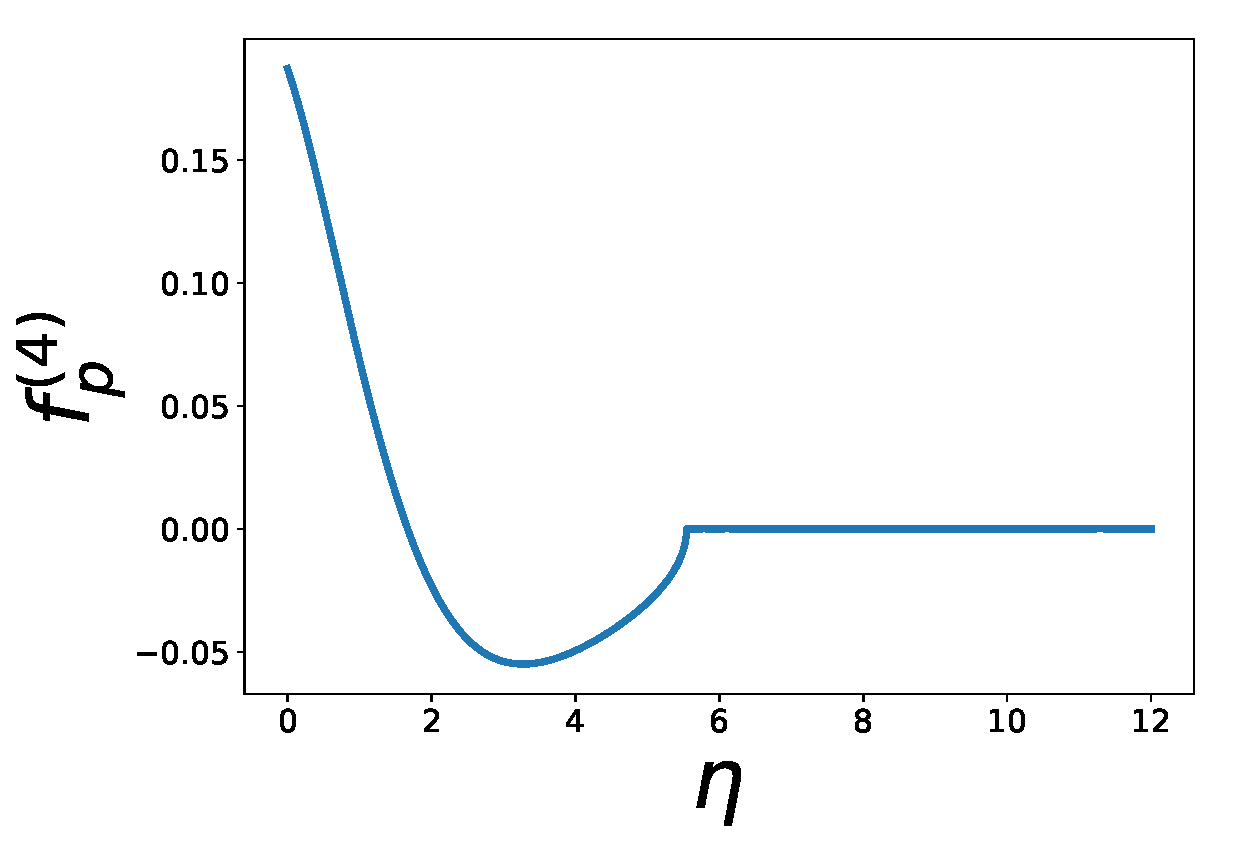
\includegraphics[width=0.6\linewidth]{new_thickening_deriv.eps}
    \caption{Fourth derivative, $f_p^{(4)}$, of the solution plotted vs $\eta$ for shear-thickening case. Typical discontinuity in the 5th derivative observed in the Sakiadis solution corresponding to the separatrix solution found in Figure~\ref{fig:shooting_thick} for $\alpha=1.4$. The discontinuity shown occurs at the edge of the finite-thickness boundary layer.}
    \label{fig:thickbest}
\end{figure}


\section{Comparative Self-Similar and Carreau Model Predictions of Wall Shear-Rates}

\hspace{\parindent} We now compare wall shear rate predictions for Newtonian, power-law, and Carreau fluids.  To do so, we express the wall shear expressions ((\ref{pl_dimensional_wall_shear}), (\ref{newtonian_dimensional_wall_shear}), and (\ref{carreau_wall_shear_dimensional_expression})) in dimensionless form using Newtonian scalings. Denoting dimensionless quantities with an overbar, we write \begin{equation}
    \bar{\tau}_i = \dfrac{\tau_i}{\rho U^2} \hphantom{\sum\sum} \mathrm{for}~~i=n, c, p,
\end{equation} where the subscripts denote the Newtonian, Carreau, and Power-Law wall shear-rates, respectively. For a Newtonian fluid with viscosity $\mu_0$, we obtain \begin{equation}
    \bar{\tau}_n = \kappa_n \operatorname{Re}_{n, x}^{-1/2}, ~~~~\kappa_n = f_p''(0; 1), \label{newtwsexpnondim}
\end{equation} where the local Newtonian Reynolds number, $ \operatorname{Re}_{n, x}$, is expressed as \begin{equation} \operatorname{Re}_{n, x} = \rho xU/\mu_0. \label{newtonian_reynolds_number}\end{equation}

\noindent For a power-law fluid ((\ref{power_law_constitutive_equation})) with consistency coefficient given by (\ref{carreau_power_law_limit_constistency_parameter})  (that relates power law and Carreau parameters to facilitate comparison), the dimensionless wall shear is expressed as \begin{equation}
    \bar{\tau}_p = \kappa_p^\alpha \operatorname{De}^{(\alpha-1)/(\alpha+1)} \operatorname{Re}_{n, x}^{-\alpha/(\alpha+1)}, ~~~~ \kappa_p = f_p''(0; \alpha),  \label{plwsexpnondim}
\end{equation} where $\operatorname{De}$ is the Deborah number given by \begin{equation}
    \operatorname{De} = \frac{\rho \lambda U^2}{\mu_0}.
\end{equation} Finally, using the Newtonian scaling, the nondimensional Carreau wall shear is given by \begin{equation} \bar{\tau}_{c} = \kappa_{c} \operatorname{Re}_{n, x}^{-1/2} \left( 1 +  \kappa_c^2\delta \right)^{(\alpha-1)/2}, ~~~~ \kappa_c=f_c''(0; \delta), \label{carwsexpnondim}\end{equation} where $\operatorname{Re}_{n,x}$ is the local Newtonian Reynolds number as in (\ref{newtonian_reynolds_number}). In (\ref{carwsexpnondim}), we note that the quantity multiplying $\kappa_c^2$ is in fact the parameter $\delta$ identified in equation (\ref{delta_definition}), which can be rewritten as  \begin{equation} \delta = \dfrac{\operatorname{De}^2}{\operatorname{Re}_{n, x}}. \end{equation} Recall that this parameter explicitly appears as the location-dependent relaxation time parameter in the Carreau model BVP (\ref{carreau_ode_form_ode}), and thus provides an explicit link to that behavior.


\begin{figure}
    \centering
    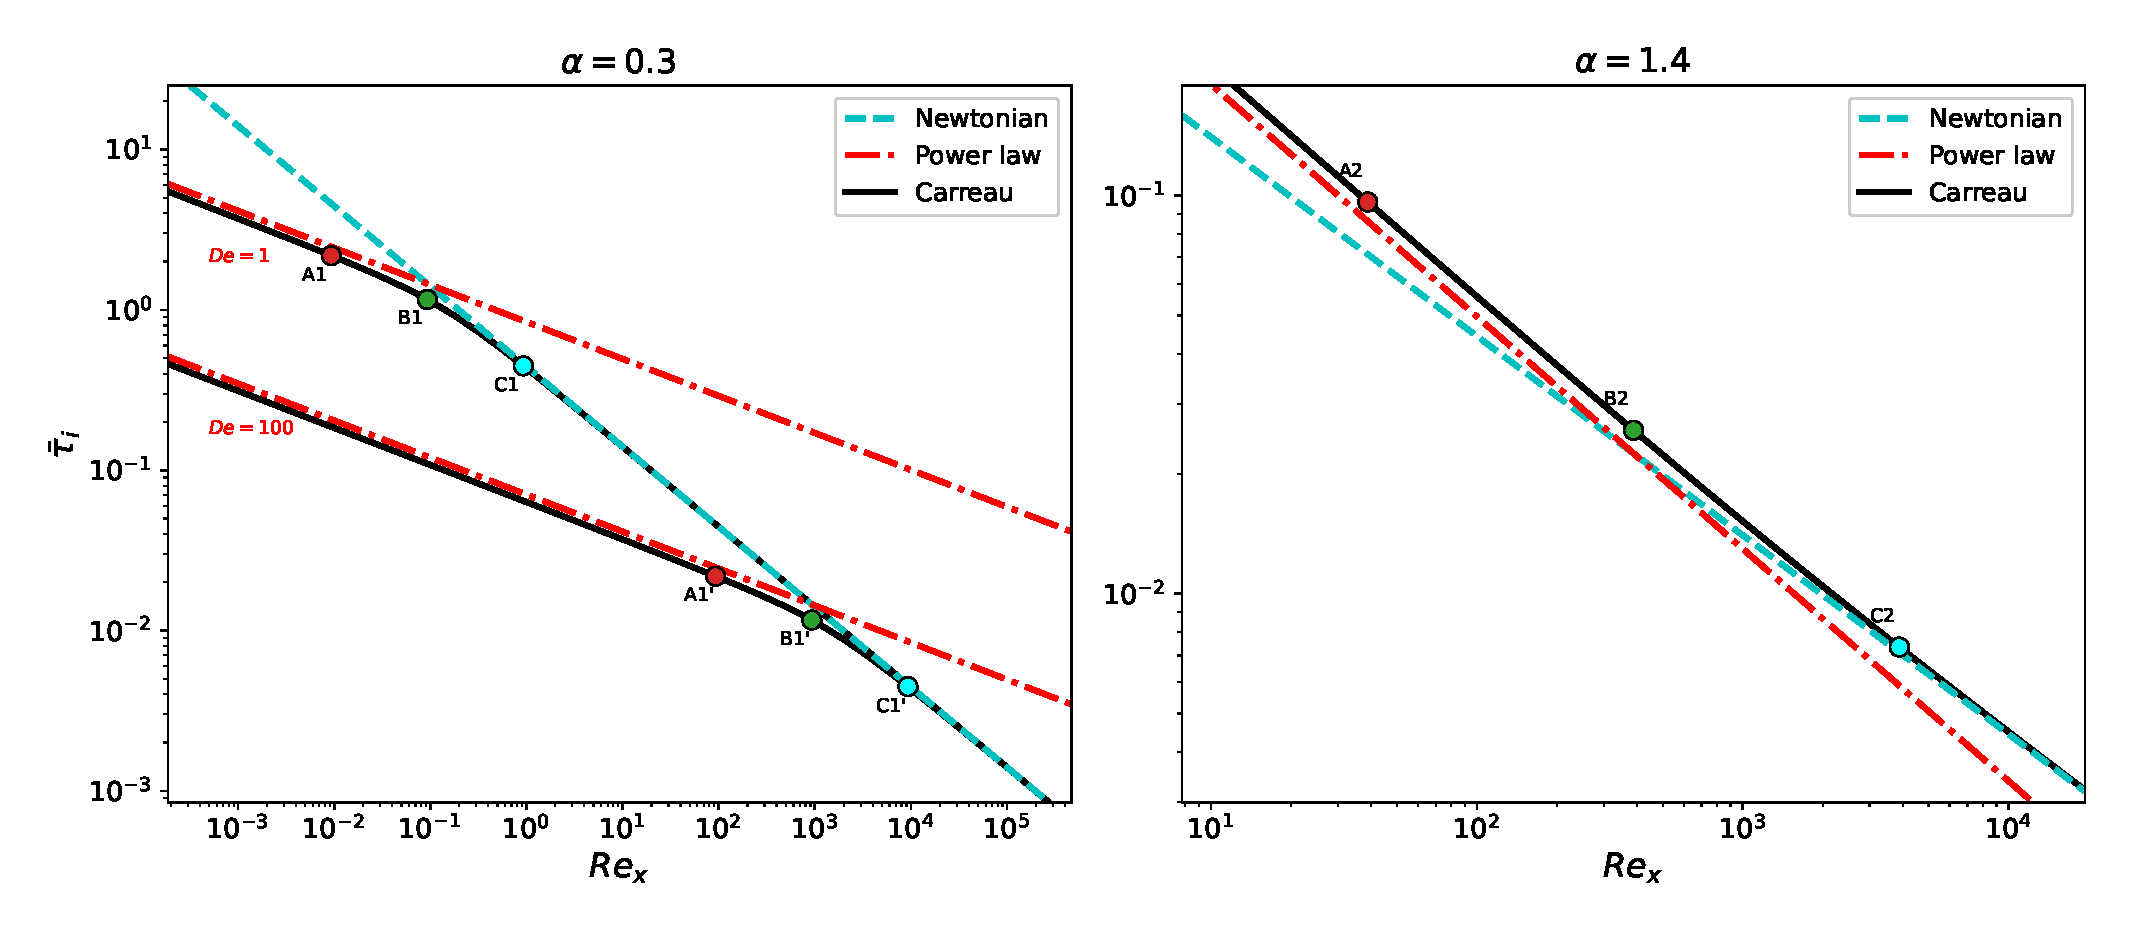
\includegraphics[width=0.9\linewidth]{new_shear.eps}
    
\includegraphics[width=0.9\linewidth]{new_shear_blas.eps}
    \caption{Wall shear for Sakiadis (top) and Blasius (bottom) boundary layers for different power-law exponent $\alpha$ for shear-thinning ($\alpha < 1$) and shear-thickening ($\alpha > 1$) regimes, for various Deborah number $\operatorname{De}$ (in the shear-thickening plots, the case $\operatorname{De}=100$ is shown). The labeled circles denote various Deborah and Reynolds number combinations referred to in Figure~\ref{fig:profiles} to follow.}
    \label{fig:wallshearfig}
\end{figure}

With the above definitions, we can directly compare the wall shear rate expressions for different models as a function of $\operatorname{Re}_{n, x}$ and $\operatorname{De}$. Figure~\ref{fig:wallshearfig} shows typical comparisons of local wall shear-rate predictions for Sakiadis and Blasius flows for shear-thinning and shear-thickening fluids. The generic behavior is that for low Reynolds number (near the front of the wall where shear rates are high) the wall shear-rate from the power law model (\ref{plwsexpnondim}), shown as a straight line in Figure 8, follows that of the Carreau model, with a slight overprediction of the Carreau behavior by the power-law model in the shear-thinning case and underprediction in the shear-thickening case. Further downstream along the wall (increasing Reynolds number), where shear rates are lower, the fluid is approximately Newtonian, and the wall shear-rates from the Carreau model approach the Newtonian limit; note that on a log-log scale, the slope of the  Newtonian curve is -1/2. The wall shear-rate for a Carreau fluid roughly follows the power-law behavior near the front of the plate until the power-law line intersects the Newtonian asymptote; beyond this transition, the Carreau wall shear closely agrees with the associated Newtonian prediction.

The behaviors discussed in Figure 8 are now discussed in more detail. In particular,  for $\operatorname{Re}_{n,x} \to \infty $, (\ref{delta_definition}) indicates that the system (\ref{carreau_ode_form_full_system}) becomes identical to the Newtonian system (\ref{power_law_ode_general}) (for $\alpha=1$).  Thus $\kappa_c \to \kappa_n$ in this limit, and thus\begin{equation}
    \bar{\tau}_c \sim \bar{\tau}_n \hphantom{\sum\sum} \mathrm{as}~~\operatorname{Re}_{n, x} \to \infty. \label{newt_lim}
\end{equation} By contrast, a comparison of power law and Carreau wall shear expressions (\ref{plwsexpnondim}) and (\ref{carwsexpnondim}) are not as straightforward to interpret. This is partially a result of the Newtonian scaling used in the dimensionless representation.  That said, one would expect the power-law approximation to the wall shear to be excellent near the leading edge of the wall ($\operatorname{Re}_{n, x} \to 0$) as the shear rate experienced is high in that region.  However, we find that \begin{equation}
    \bar{\tau}_c \sim (1 - c(\alpha)) \bar{\tau}_p \hphantom{\sum\sum} \mathrm{as}~~\operatorname{Re}_{n, x} \to 0. \label{cdef}
\end{equation} where $c(\alpha)$ is a finite correction function, i.e., there is an observable offset between the power-law and Carreau model lines in Figure 8 as $\operatorname{Re}_{n, x} \to 0$  for both Sakiadis and Blasius flows.  Figure~\ref{fig:ws_front_err_proof} shows the typical dependence of the magnitude of the error between power law and Carreau model predictions for Sakiadis flow over a range of $\operatorname{Re}_{n, x}$. As indicated, the relative error between $\tau_c$ and $\tau_p$ is dependent on $\operatorname{De}$ at finite $\operatorname{Re}_x$, but becomes independent of $\operatorname{De}$ as $\operatorname{Re}_x \to 0$; this justifies the dependence of the correction function $c(\alpha)$ only on $\alpha$ in (\ref{cdef}).

Figure~\ref{fig:c_plot} provides a plot of $c(\alpha)$ for Blasius and Sakiadis flows. In accordance with (\ref{newt_lim}), we find that $c(\alpha) \to 0$ as $\alpha \to 1$.  On the other hand, Figure~\ref{fig:c_plot} indicates that for the range $\alpha \in [0.3, 1.4]$ the power-law model predicts the Carreau wall shear as $\operatorname{Re}_{n, x} \to 0$ with an error of at most approximately 10\%, for both the Blasius and Sakiadis configurations. It is notable that the Blasius correction is almost identical to that of Sakiadis. We do not have a precise explanation for this, although it suggests that the rheology near the wall is dominating the error $c(\alpha)$.

\begin{figure}
    \centering
    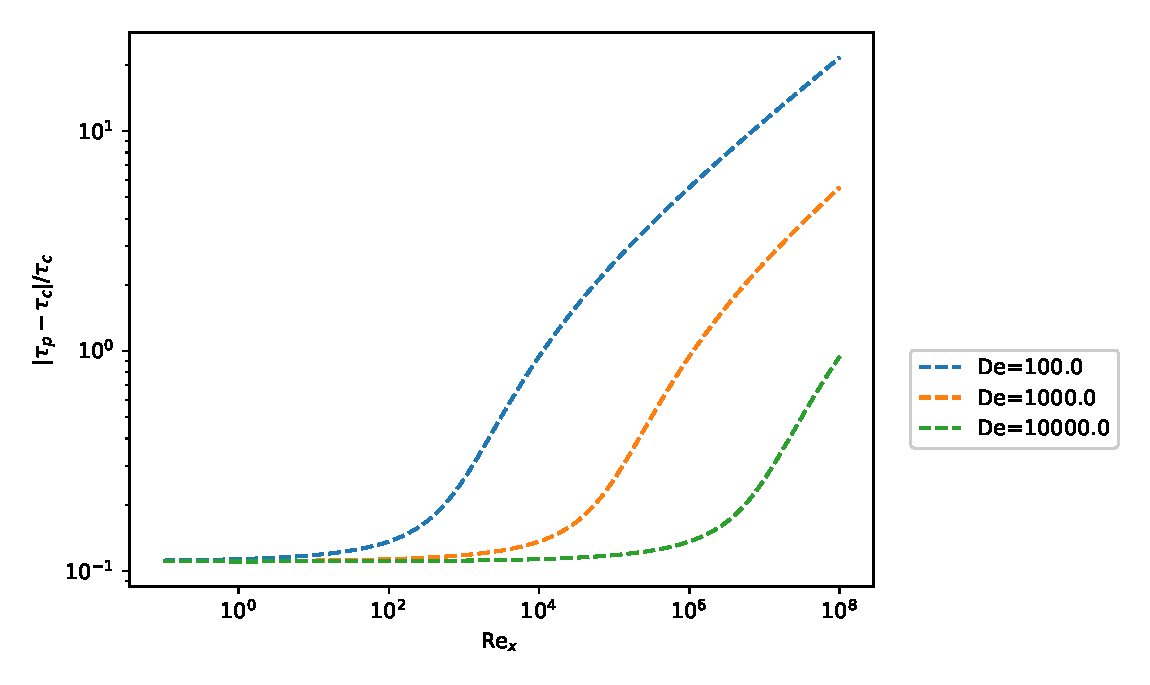
\includegraphics[width=.8\linewidth]{rel_err.eps}
    \caption{Error in wall shear predictions near the front of the plate for $\alpha = 0.3$ for the Sakiadis flow for various Deborah numbers.}
    \label{fig:ws_front_err_proof}
\end{figure}

\begin{figure}
    \centering
    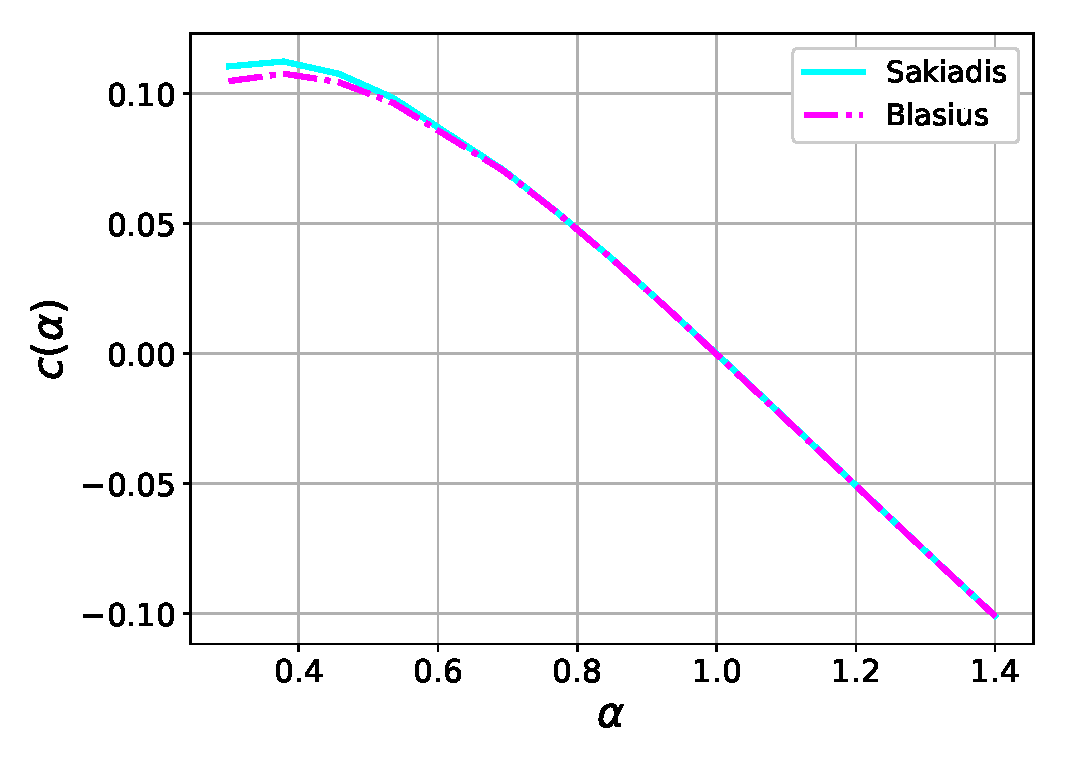
\includegraphics[width=0.8\linewidth]{fig7.eps}
    \caption{The dependence of the correction function $c(\alpha)$ in (\ref{cdef}) as a function of the power law exponent alpha, for Sakaidis (top) and Blasius (bottom) flows}
    \label{fig:c_plot}
\end{figure}


\section{Discussion}

\subsection{The Effect of Velocity Profiles on Wall Shear-Rates}

\hspace{\parindent}As $\eta \to \infty$ in the Carreau BVP (\ref{carreau_ode_form_full_system}), the shear rate approaches zero in the Blasius and Sakiadis flows.  Thus, the Carreau fluid flow transitions to Newtonian in those regions in accordance with the rheological curve shown in Figure \ref{fig:rheology}. However, for a power-law fluid, the viscosity continues to change as $\eta \to \infty$ depending on the value of $\alpha$; for a shear-thinning fluid ($\alpha<1$), the viscosity approaches infinity, and for a shear-thickening fluid ($\alpha>1$), the viscosity approaches zero in accordance with (\ref{power_law_constitutive_equation}).  Thus, in the far field away from the wall, the behavior of the velocity profiles is expected to be different. To understand the implications of this result we examine the well-known expression for the wall shear-rate that arises upon integration of the boundary layer equations (\ref{blsystem}) over the domain from $y=0$ to infinity (see Figure 2).  Such a procedure is embedded in the classical Polhausen approximation for Blasius \citep{Schlichting} and Sakiadis \citep{Sakiadis1961a} flows.  Regardless of viscosity model, the integration of (\ref{blsystem}) for the Blasius problem yields \begin{equation}
    \bar{\tau}_i = \frac{\text{d}}{\text{d}x} \int_0^\infty u_x(U-u_x) ~ \text{d}y \hphantom{\sum\sum} i = n, c, p. \label{schlic} \end{equation} An equivalent expression for the Sakiadis problem is obtained by taking $U=0$ in (\ref{schlic}). Equation (\ref{schlic}) indicates that the \textit{complete} velocity field affects the wall shear---not just the local shear-rate at the wall.  This result is perhaps expected, since all of the boundary-layer problems we have solved are indeed boundary-value problems over their computational domains.  It thus suffices, then, to compare velocity profiles for power law, Newtonian, and Carreau models at various values of $\operatorname{Re}_{n, x}$ to understand the nature of the agreement of wall shears in various locations along the wall (as seen in Figure 8) and the origin of the nonzero value of $c(\alpha)$ in (\ref{cdef}).

\begin{figure}
    \centering
    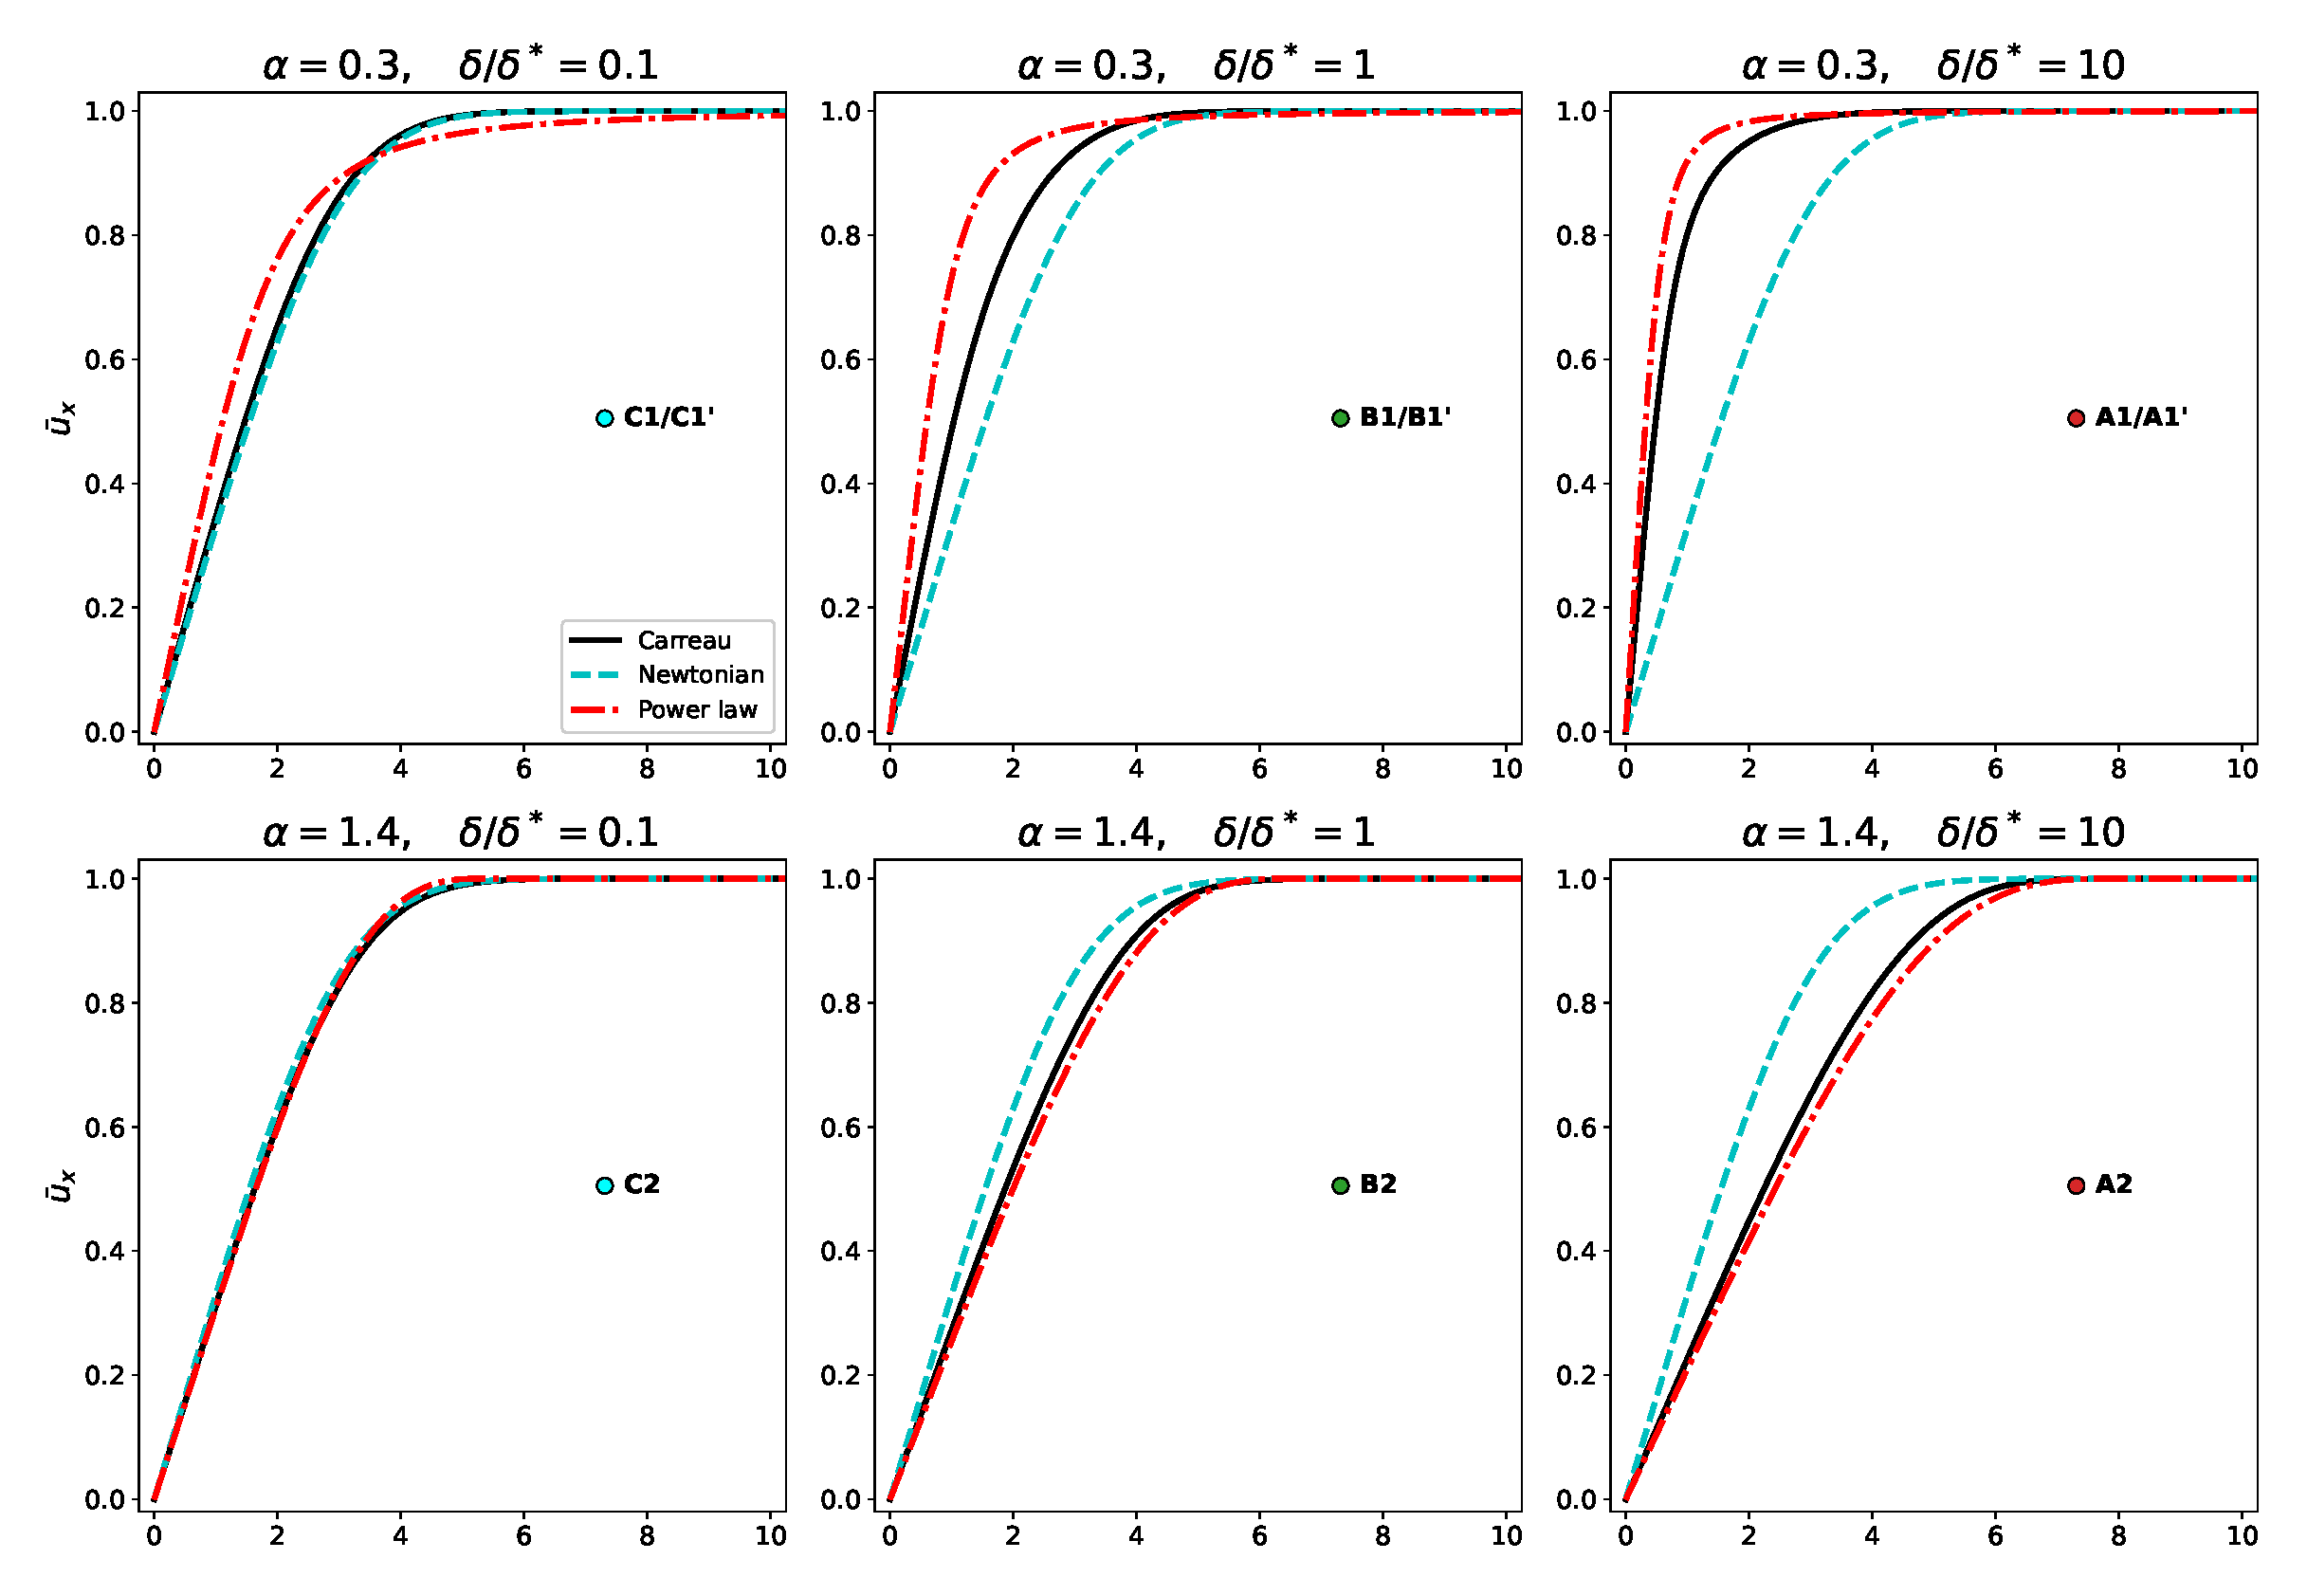
\includegraphics[width=0.8\linewidth]{new_profiles_blas.eps}
    
\includegraphics[width=0.8\linewidth]{new_profiles.eps}
    \caption{Dimensionless velocity profiles plotting $\bar{u}_x = u_x/U$ for the self-similar and Carreau viscosity models for a typical shear-thinning fluid at an intermediate distance along the wall for the Blasius (Top 2 rows) and Sakiadis (Bottom 2 rows).}
    \label{fig:profiles}
\end{figure}

Figure \ref{fig:profiles} provides comparisons of dimensionless velocity profiles for the power-law, Newtonian, and Carreau models corresponding to various locations along the wall for both Sakiadis and Blasius flow---this is characterized by the parameter $\delta$ in (\ref{carreau_ode_form_full_system}) for the Carreau fluid, and according to (\ref{delta_definition}), the value of $\operatorname{Re}_{n, x}$ for a given $\operatorname{De}$. The velocity profiles in Figure \ref{fig:profiles} correspond to the indicated points in Figure \ref{fig:wallshearfig}.  Points labeled similarly with and without a prime correspond to the same value of $\delta$ in (\ref{delta_definition}).  As the solution for $f_c$ in (\ref{carreau_ode_form_full_system}) is only a function of $\delta$ for a given value of $\alpha$, dimensionless velocity profiles will be identical for the same value of $\delta$.  Additionally, in the figures themselves, a ratio of $\delta/\delta^*$ is referenced.  Here, $\delta^*$ corresponds to the intersection of the Newtonian and power-law lines on the plots; an expression for this intersection is provided in equation (\ref{delta_definition}) in section (5.2).  Here, the key physics is that for $\delta/\delta^* \ll 1$, the Carreau model wall shear-rates agree with those of the Newtonian model in Figure \ref{fig:wallshearfig}; for $\delta/\delta^* \gg 1$, the Carreau model wall shear-rates follow those for a power-law fluid.  So, a comparison of velocity profiles for these values of $\delta$ reveal the sensitivity of wall shear-rate to the global behavior of the velocity field according to (\ref{schlic}).

For velocity profiles corresponding to the red points in Figure \ref{fig:wallshearfig}, the shear rates are clearly in the power law region.  Accordingly, we observe that although the slope of the velocity field near the wall is similar for these points, the velocity profile away from the wall is not, relative to the error in the wall shear-rate.  According to equation (\ref{schlic}) (with $U=0$ for the Sakiadis flow), this accounts for the error $c(\alpha)$ in (\ref{cdef}). Note that far downstream (indicated as blue points in Figure \ref{fig:wallshearfig}) where the flow is truly Newtonian (large value of $\operatorname{Re}_{n, x}$), the profiles between the Newtonian and Carreau model agree. We note that the slope of the velocity profiles, which can be directly related to shear parameters $\kappa_p$ and $\kappa_c$, is closely matched between power-law and Carreau fluids in regions where the shear rates match closely (but not exactly according to (\ref{cdef})).  This indicates that much, but not all, of the shear rate behavior is governed by the velocity profile at the wall---as evidenced by the nonzero value of $c(\alpha)$ in these regions.

We point out the work of \citet{Dabrowski}, who considered the origin of the breakdown in the smoothness of the solution to the full Blasius boundary layer problem for shear-thickening power-law fluids. They point out that this can be seen as a breakdown in the boundary layer equations. For a shear-thickening power-law fluid, the fluid is approximately inviscid far from the wall since the shear-rate is small there. The Carreau solution, which is well-behaved far from the wall, avoids this issue because the fluid viscosity approaches the Newtonian plateau $\mu_0$ in the low-shear limit; our calculated solutions for the Carreau model are completely smooth in this regime. Note that Denier and Dabrowski find that a continuous solution can be recovered by introducing a ``viscous diffusion layer'' in which viscous effects from shear not normal to the wall become relevant, effectively recovering a more viscous response in that regime. Here, we have shown that such a modification to the governing equation is not required; rather, restoring the appropriate Newtonian behavior in the low shear limit can enable an adequate solution.

\subsection{Approximation Accuracy For Wall Shear}



\hspace{\parindent}If we take $\alpha \sim 0.3$  to $\alpha \sim 1.4$ as a reasonable range on power-law behaviors typically encountered, Figure~\ref{fig:c_plot} and Equation (\ref{cdef}) indicate that the error in wall shear-rate when it is used an approximation for the true (Carreau) behavior is $\sim 11\%$ as $\operatorname{Re}_{n, x} \to 0$. In practice, such an error is smaller in absolute and relative terms than the shear-rate error incurred near the transition region where the rheology switches from power-law to Newtonian as shown in Figure~\ref{fig:wallshearfig}  (these are the regions in the vicinity of labeled points with green circles in the figure). In the Newtonian region, the Carreau and Newtonian wall shear-rates appear to match asymptotically as $\operatorname{Re}_{n, x} \to \infty$.  Thus, from an engineering perspective, the power law and Newtonian asymptotes, such as shown in Figure \ref{fig:wallshearfig} are well-predictive of Carreau wall shear, while for greater accuracy, one can still solve the one-parameter family of ODEs (\ref{carreau_ode_form_full_system}) to obtain the full Carreau solution.

The transition region between Newtonian and power-law behavior is found to occur where the wall shear-rate curves intersect, as shown in Figure \ref{fig:wallshearfig}. Since the power-law and Newtonian wall shear asymptote predictions are self-similar, their intersection may be used as a guide to using the self similar solutions most efficiently together---without solving the Carreau model system numerically. Setting (\ref{plwsexpnondim}) equal to (\ref{newtwsexpnondim}), this crossover is found to occur at a critical value of $\delta$, denoted $\delta^*$, which is related to $\kappa_n$ and $\kappa_p$ (both functions of $\alpha$) as \begin{equation} \delta^* = \left(\dfrac{\kappa_p^\alpha}{\kappa_n}\right)^{2\frac{1+\alpha}{1-\alpha}}.\end{equation} It is seen that over a large range of alpha from 0 to 2, $\delta^*$ changes from 14 to 20; i.e., its value is relatively insensitive to $\alpha$.

As an application of this result, a good approximation can be made to integrated quantities derived from the Carreau wall shear (which is not self-similar) by using the appropriate self-similar model in each regime. For example, suppose one wanted to know the drag on the plate exerted by the boundary layer over some large length of plate. This may be obtained exactly by integrating (\ref{carreau_wall_shear_dimensional_expression}) in dimensional form over the entire domain. Alternatively, using the known value of $\delta^*$ corresponding to a given $\alpha$, we can deduce a critical $x^*$ in closed form, before which the shear is approximately power-law and after which it is approximately Newtonian. Since the shear in both of those cases scales as a power of $x$, breaking the integral of $\tau_c$ into two pieces yields an accurate estimate of the drag on the plate with essentially no computational work beyond looking up $\kappa_p$, even for the much more difficult non-self-similar Carreau Sakiadis or Blasius boundary layer. Additionally, if the wall is small enough, for $\delta<\delta^*$, the power law model may be used approximately across the entire wall, if the identified error $c(\alpha)$ is acceptable.



\section{Conclusion}

The present work investigated the boundary layer flows of a non-Newtonian fluid over a flat plate, focusing on both the Sakiadis and Blasius boundary layers. While the physically realistic Carreau viscosity model does not admit self-similar solutions, the wall shear predictions are well-approximated by the self-similar solutions in the Newtonian and power-law regimes. These regimes can be identified a priori from self-similar calculations alone, and the corresponding predictions are found to match the Carreau flow with a quantifiable error. This error arises in the wall shear-rates when a power-law model is used to approximate Carreau model behavior in the high-shear region near the front of the plot, and yet further error corresponding to the intermediate region where the flow switches from a power-law to a Newtonian rheology. The former error owes to differences in the velocity fields away from the wall, even in regimes where the shear rate behavior is largely affected by the local shear rate at the wall. There are no contributions to wall shear errors when a Newtonian model is used in regions along the wall where wall shear is low---the Carreau and Newtonian models agree asymptotically in such regions. To within quantifiable errors in the power law regime, self-similar solutions do provide reliable wall shear estimates, and this framework was found to apply for both the Sakiadis and Blasius flows across a wide range of rheologies. For cases where this error is acceptable in applications, we identify a dimensionless criterion that allows both similarity solutions to be used in place of Carreau wall shear rate predictions. These conclusions hold for all shear-thinning and thickening cases examined for Blasius and Sakiadis flows.


As part of this study, we identified new power law solutions for the Sakiadis flow for shear thinning and thickening cases, and these solutions are consistent with the wall shear predictions in the power-law regime of the Carreau model.

\section*{Acknowledgements}

This work was supported by the U.S. Department of Energy, Office of Science, Basic Energy Sciences, under Award \# DE-SC0025300.

\bibliographystyle{jfm}
\bibliography{biblio}

\end{document}
